%%
% The BIThesis Template for Bachelor Graduation Thesis
%
% 北京理工大学毕业设计(论文) —— 使用 XeLaTeX 编译
%
% Copyright 2021 BITNP
%
% This work may be distributed and/or modified under the
% conditions of the LaTeX Project Public License, either version 1.3
% of this license or (at your option) any later version.
% The latest version of this license is in
%   http://www.latex-project.org/lppl.txt
% and version 1.3 or later is part of all distributions of LaTeX
% version 2005/12/01 or later.
%
% This work has the LPPL maintenance status `maintained'.
%
% The Current Maintainer of this work is Feng Kaiyu.
%
% Compile with: xelatex -> biber -> xelatex -> xelatex

% 章节支持、单面打印:ctexbook
\documentclass[bachelor,footskip=24pt]{bitbook}
% 如果想要修改样式,但无法找到样式在哪里定义:请参考 https://bithesis.bitnp.net/Guide/4-Others/Troubleshooting.html#%E6%83%B3%E8%A6%81%E4%BF%AE%E6%94%B9%E9%83%A8%E5%88%86%E6%A0%B7%E5%BC%8F-%E4%BD%86%E6%98%AF%E6%89%BE%E4%B8%8D%E5%88%B0%E6%A0%B7%E5%BC%8F%E5%9C%A8%E5%93%AA%E9%87%8C%E5%AE%9A%E4%B9%89

% 另一个临时的“修改页眉文字”的解决方法(非常不优雅,只作为临时措施)。
% 请注释掉以下 20 行内容使用。
 % 从原有主题继承自定义主题
 \fancypagestyle{BIThesisCustom}[BIThesis]{
   % 定义页眉、页码
   \fancyhead[C]{\zihao{4}\ziju{0.08}\songti{北京理工大学汇编接口小组项目实验报告}}
 }
 % 设置章节格式
 \ctexset{chapter={
     pagestyle = BIThesisCustom,
   }
 }
 % 前置页面(原创性声明、中英文摘要、目录等)
 \renewcommand{\frontmatter}{
   \pagenumbering{Roman}
   \pagestyle{BIThesisCustom}
 }
 % 正文页面
 \renewcommand{\mainmatter}{
   \pagenumbering{arabic}
   \pagestyle{BIThesisCustom}
 }
% ------------------------------------------------------------------

% 使用 listings 宏包进行代码块使用,并使用了预定义的样式,
% 你也可以选用自己的喜欢的其他宏包,如 minted;
% 然而由于 minted 依赖 Python 的 Pygments 库作为外部依赖,因此出于模板的建议性考虑,我们没有提供 minted 进行代码块书写的示例。
% 但是,我们仍旧非常建议你使用 minted。
\usepackage{listings}

% 参考文献引用文件位于 misc/ref.bib
\addbibresource{misc/ref.bib}

% 在这里填写你的论文中英文题目
\newcommand{\thesisTitle}{北京理工大学汇编接口小组项目实验报告}
\newcommand{\thesisTitleEN}{Compiling the experimental report of interface group project of Beijing Institute of Technology}

% 在这里填写你的相关信息
\newcommand{\deptName}{计算机学院}
\newcommand{\majorName}{计算机科学与技术}
\newcommand{\yourName}{杨汶锦、王岩、蒙思洁、吴一凡}
\newcommand{\yourStudentID}{1120193624、27、02、32}
\newcommand{\mentorName}{张全新}
% 如果你的毕设为校外毕设,请将下面这一行语句解除注释(删除第一个百分号字符)并在第二组花括号中填写你的校外毕设导师名字
% \newcommand{\externalMentorName}{左偏树}

% 文档开始
\begin{document}

% 标题页面:如无特殊需要,本部分无需改动
%%
% The BIThesis Template for Bachelor Graduation Thesis
%
% 北京理工大学毕业设计(论文)封面页 —— 使用 XeLaTeX 编译
%
% Copyright 2020-2021 BITNP
%
% This work may be distributed and/or modified under the
% conditions of the LaTeX Project Public License, either version 1.3
% of this license or (at your option) any later version.
% The latest version of this license is in
%   http://www.latex-project.org/lppl.txt
% and version 1.3 or later is part of all distributions of LaTeX
% version 2005/12/01 or later.
%
% This work has the LPPL maintenance status `maintained'.
%
% The Current Maintainer of this work is Feng Kaiyu.
%
% 封面
%
% 如无特殊需要,本页面无需更改

% Underline new command for student information
% Usage: \dunderline[<offset>]{<line_thickness>}
\newcommand\dunderline[3][-1pt]{{%
  \setbox0=\hbox{#3}
  \ooalign{\copy0\cr\rule[\dimexpr#1-#2\relax]{\wd0}{#2}}}}

% Cover Page
\begin{titlepage}
  \makeatletter
  \@ifundefined{externalMentorName}{
    % 校内毕设封面顶部间距
    \vspace*{19mm}
  }{
    % 校外毕设封面顶部间距
    \vspace*{13mm}
  }
  \centering

  
\includegraphics[width=9.87cm]{images/header.png}

  \vspace*{-3mm}

  \zihao{-0}\textbf{\ziju{0.12}\songti{汇编接口上机实验报告}}

  \vspace{16mm}

  \zihao{2}\textbf{\xihei\thesisTitle}

  \vspace{3mm}

  \begin{spacing}{1.2}
    \zihao{3}\selectfont{\textbf{\thesisTitleEN}}
  \end{spacing}

  \vspace{15mm}

  \flushleft

  \makeatletter
  \@ifundefined{externalMentorName}{
    % 生成校内毕设封面字段
    \makeatother
    \begin{spacing}{1.8}
      \hspace{27mm}\songti\zihao{3}\selectfont{学\hspace{11mm}院:\dunderline[-10pt]{1pt}{\makebox[78mm][c]{\deptName}}}

      \hspace{27mm}\songti\zihao{3}\selectfont{专\hspace{11mm}业:\dunderline[-10pt]{1pt}{\makebox[78mm][c]{\majorName}}}

      \hspace{27mm}\songti\zihao{3}\selectfont{学生姓名:\dunderline[-10pt]{1pt}{\makebox[78mm][c]{\yourName}}}

      \hspace{27mm}\songti\zihao{3}\selectfont{学\hspace{11mm}号:\dunderline[-10pt]{1pt}{\makebox[78mm][c]{\yourStudentID}}}

      \hspace{27mm}\songti\zihao{3}\selectfont{指导教师:\dunderline[-10pt]{1pt}{\makebox[78mm][c]{\mentorName}}}
    \end{spacing}
  }{
    % 生成校外毕设封面字段
    \makeatother
    \begin{spacing}{1.8}
      \hspace{19.4mm}\songti\zihao{3}\selectfont{学\hspace{19.6mm}院\hspace{3mm}:\dunderline[-10pt]{1pt}{\makebox[77.4mm][c]{\deptName}}}

      \hspace{19.4mm}\songti\zihao{3}\selectfont{专\hspace{19.6mm}业\hspace{3mm}:\dunderline[-10pt]{1pt}{\makebox[77.4mm][c]{\majorName}}}

      \hspace{19.4mm}\songti\zihao{3}\selectfont{学\hspace{2.8mm}生\hspace{2.8mm}姓\hspace{2.8mm}名\hspace{3mm}:\dunderline[-10pt]{1pt}{\makebox[77.4mm][c]{\yourName}}}

      \hspace{19.4mm}\songti\zihao{3}\selectfont{学\hspace{19.6mm}号\hspace{3mm}:\dunderline[-10pt]{1pt}{\makebox[77.4mm][c]{\yourStudentID}}}

      \hspace{19.4mm}\songti\zihao{3}\selectfont{指\hspace{2.8mm}导\hspace{2.8mm}教\hspace{2.8mm}师\hspace{3mm}:\dunderline[-10pt]{1pt}{\makebox[77.4mm][c]{\mentorName}}}

      \hspace{19.4mm}\songti\zihao{3}\selectfont{校外指导教师:\dunderline[-10pt]{1pt}{\makebox[77.4mm][c]{\externalMentorName}}}
    \end{spacing}
  }

  \vspace*{\fill}
  \centering
  \zihao{3}\ziju{0.5}\songti{\today}
\end{titlepage}


% 前置页面定义
\frontmatter
% 原创性声明:如无特殊需要,本部分无需改动
% 更改为 PDF 页面插入,如需要添加内容,可考虑先用 Word 制作再覆盖 misc/1_originality.pdf
%
\includepdf{misc/1_originality.pdf}
\newpage
%%%
% The BIThesis Template for Bachelor Graduation Thesis
%
% 北京理工大学毕业设计(论文)原创性声明页 —— 使用 XeLaTeX 编译
%
% Copyright 2020-2021 BITNP
%
% This work may be distributed and/or modified under the
% conditions of the LaTeX Project Public License, either version 1.3
% of this license or (at your option) any later version.
% The latest version of this license is in
%   http://www.latex-project.org/lppl.txt
% and version 1.3 or later is part of all distributions of LaTeX
% version 2005/12/01 or later.
%
% This work has the LPPL maintenance status `maintained'.
%
% The Current Maintainer of this work is Feng Kaiyu.
%
% 如无特殊需要,本页面无需更改

% 原创性声明页无页码页面格式
\fancypagestyle{originality}{
  % 页眉高度
  \setlength{\headheight}{20pt}

  % 页眉和页脚(页码)的格式设定
  \fancyhf{}
  \fancyhead[C]{\zihao{4}\ziju{0.08}\songti{北京理工大学本科生毕业设计(论文)}}

  % 页眉分割线稍微粗一些
  \renewcommand{\headrulewidth}{0.6pt}
}

\pagestyle{originality}
\topskip=0pt

% 圆形数字编号定义
\newcommand{\circled}[2][]{\tikz[baseline=(char.base)]
  {\node[shape = circle, draw, inner sep = 1pt]
  (char) {\phantom{\ifblank{#1}{#2}{#1}}};
  \node at (char.center) {\makebox[0pt][c]{#2}};}}
\robustify{\circled}

% 设置行间距
\setlength{\parskip}{0.4em}
\renewcommand{\baselinestretch}{1.41}

% 顶部空白
\vspace*{-6mm}

% 原创性声明部分
\begin{center}
  \heiti\zihao{2}\textbf{原创性声明}
\end{center}

% 本部分字号为小三
\zihao{-3}

本人郑重声明:所呈交的毕业设计(论文),是本人在指导老师的指导下独立进行研究所取得的成果。除文中已经注明引用的内容外,本文不包含任何其他个人或集体已经发表或撰写过的研究成果。对本文的研究做出重要贡献的个人和集体,均已在文中以明确方式标明。

特此申明。

\vspace{13mm}

\begin{flushright}
  本人签名:\hspace{40mm}日\hspace{2.5mm}期:\hspace{13mm}年\hspace{8mm}月\hspace{8mm}日
\end{flushright}

\vspace{17mm}

% 使用授权声明部分
\begin{center}
  \heiti\zihao{2}\textbf{关于使用授权的声明}
\end{center}

本人完全了解北京理工大学有关保管、使用毕业设计(论文)的规定,其中包括:\circled{1}学校有权保管、并向有关部门送交本毕业设计(论文)的原件与复印件;\circled{2}学校可以采用影印、缩印或其它复制手段复制并保存本毕业设计(论文);\circled{3}学校可允许本毕业设计(论文)被查阅或借阅;\circled{4}学校可以学术交流为目的,复制赠送和交换本毕业设计(论文);\circled{5}学校可以公布本毕业设计(论文)的全部或部分内容。

\vspace*{1mm}

\begin{flushright}
  \begin{spacing}{1.65}
    \zihao{-3}
    本人签名:\hspace{40mm}日\hspace{2.5mm}期:\hspace{13mm}年\hspace{8mm}月\hspace{8mm}日\\
    指导老师签名:\hspace{40mm}日\hspace{2.5mm}期:\hspace{13mm}年\hspace{8mm}月\hspace{8mm}日
  \end{spacing}
\end{flushright}

\newpage

% 摘要:在摘要相应的 TeX 文件处进行摘要部分的撰写
%%%
% The BIThesis Template for Bachelor Graduation Thesis
%
% 北京理工大学毕业设计(论文)中英文摘要 —— 使用 XeLaTeX 编译
%
% Copyright 2020-2021 BITNP
%
% This work may be distributed and/or modified under the
% conditions of the LaTeX Project Public License, either version 1.3
% of this license or (at your option) any later version.
% The latest version of this license is in
%   http://www.latex-project.org/lppl.txt
% and version 1.3 or later is part of all distributions of LaTeX
% version 2005/12/01 or later.
%
% This work has the LPPL maintenance status `maintained'.
%
% The Current Maintainer of this work is Feng Kaiyu.

% 中英文摘要章节
\zihao{-4}
\vspace*{-11mm}

\begin{center}
  \heiti\zihao{-2}\textbf{\thesisTitle}
\end{center}

\vspace*{2mm}

{\let\clearpage\relax \chapter*{\textmd{摘~~~~要}}}
\addcontentsline{toc}{chapter}{摘~~~~要}
\setcounter{page}{1}

\vspace*{1mm}

\setstretch{1.53}
\setlength{\parskip}{0em}

% 中文摘要正文从这里开始
本文……。

\textcolor{blue}{摘要正文选用模板中的样式所定义的“正文”,每段落首行缩进 2 个字符;或者手动设置成每段落首行缩进 2 个汉字,字体:宋体,字号:小四,行距:固定值 22 磅,间距:段前、段后均为 0 行。阅后删除此段。}

\textcolor{blue}{摘要是一篇具有独立性和完整性的短文,应概括而扼要地反映出本论文的主要内容。包括研究目的、研究方法、研究结果和结论等,特别要突出研究结果和结论。中文摘要力求语言精炼准确,本科生毕业设计(论文)摘要建议 300-500 字。摘要中不可出现参考文献、图、表、化学结构式、非公知公用的符号和术语。英文摘要与中文摘要的内容应一致。阅后删除此段。}

\vspace{4ex}\noindent\textbf{\heiti 关键词:北京理工大学;本科生;毕业设计(论文)}
\newpage

% 英文摘要章节
\vspace*{-2mm}

\begin{spacing}{0.95}
  \centering
  \heiti\zihao{3}\textbf{\thesisTitleEN}
\end{spacing}

\vspace*{17mm}

{\let\clearpage\relax \chapter*{
  \zihao{-3}\textmd{Abstract}\vskip -3bp}}
\addcontentsline{toc}{chapter}{Abstract}
\setcounter{page}{2}

\setstretch{1.53}
\setlength{\parskip}{0em}

% 英文摘要正文从这里开始
In order to study……

\textcolor{blue}{Abstract 正文设置成每段落首行缩进 2 字符,字体:Times New Roman,字号:小四,行距:固定值 22 磅,间距:段前、段后均为 0 行。阅后删除此段。}

\vspace{3ex}\noindent\textbf{Key Words: BIT; Undergraduate; Graduation Project (Thesis)}
\newpage

% 目录:如无特殊需要,本部分无需改动
%%
% The BIThesis Template for Bachelor Graduation Thesis
%
% 北京理工大学毕业设计(论文)目录 —— 使用 XeLaTeX 编译
%
% Copyright 2020-2021 BITNP
%
% This work may be distributed and/or modified under the
% conditions of the LaTeX Project Public License, either version 1.3
% of this license or (at your option) any later version.
% The latest version of this license is in
%   http://www.latex-project.org/lppl.txt
% and version 1.3 or later is part of all distributions of LaTeX
% version 2005/12/01 or later.
%
% This work has the LPPL maintenance status `maintained'.
%
% The Current Maintainer of this work is Feng Kaiyu.
%
% 如无特殊需要,本页面无需更改

% 目录开始

% 调整目录行间距
\renewcommand{\baselinestretch}{1.35}
% 目录
\tableofcontents
\newpage


% 正文开始
\mainmatter
% 正文 22 磅的行距
\setlength{\parskip}{0em}
\renewcommand{\baselinestretch}{1.53}
% 修复脚注出现跨页的问题
\interfootnotelinepenalty=10000

% 第一章
%%
% The BIThesis Template for Bachelor Graduation Thesis
%
% 北京理工大学毕业设计(论文)第一章节 —— 使用 XeLaTeX 编译
%
% Copyright 2020-2021 BITNP
%
% This work may be distributed and/or modified under the
% conditions of the LaTeX Project Public License, either version 1.3
% of this license or (at your option) any later version.
% The latest version of this license is in
%   http://www.latex-project.org/lppl.txt
% and version 1.3 or later is part of all distributions of LaTeX
% version 2005/12/01 or later.
%
% This work has the LPPL maintenance status `maintained'.
%
% The Current Maintainer of this work is Feng Kaiyu.
%
% 第一章节

\chapter{一级题目}

\section{二级题目}
% 这里插入一个参考文献,仅作参考
正文……\cite{yuFeiJiZongTiDuoXueKeSheJiYouHuaDeXianZhuangYuFaZhanFangXiang2008}

\subsection{三级题目}

正文……\cite{Hajela2012Application}

\textcolor{blue}{正文部分:宋体、小四;正文行距:22磅;间距段前段后均为0行。阅后删除此段。}

\textcolor{blue}{图、表居中,图注标在图下方,表头标在表上方,宋体、五号、居中,1.25倍行距,间距段前段后均为0行,图表与上下文之间各空一行。阅后删除此段。}

\textcolor{blue}{\underline{\underline{图-示例:(阅后删除此段)}}}

\begin{figure}[htbp]
  \vspace{13pt} % 调整图片与上文的垂直距离
  \centering
  
\includegraphics[]{images/bit_logo.png}
  \caption{标题序号}\label{标题序号} % label 用来在文中索引
\end{figure}

\textcolor{blue}{\underline{\underline{表-示例:(阅后删除此段)}}}

\begin{table}[htbp]
  \linespread{1.5}
  \zihao{5}
  \centering
  \caption{统计表}\label{统计表}
  \begin{tabular}{*{5}{>{\centering\arraybackslash}p{2cm}}}
    \hline
    项目    & 产量    & 销量    & 产值   & 比重    \\ \hline
    手机    & 1000  & 10000 & 500  & 50\%  \\
    计算机   & 5500  & 5000  & 220  & 22\%  \\
    笔记本电脑 & 1100  & 1000  & 280  & 28\%  \\ \hline
    合计    & 17600 & 16000 & 1000 & 100\% \\ \hline
    \end{tabular}
\end{table}

\textcolor{blue}{公式标注应于该公式所在行的最右侧。对于较长的公式只可在符号处(+、-、*、/、$\leqslant$ $\geqslant$ 等)转行。在文中引用公式时,在标号前加“式”,如式(1-2)。阅后删除此
段。}

\textcolor{blue}{公式-示例:(阅后删除此段)}
% 公式上下不要空行,置于同一个段落下即可,否则上下距离会出现高度不一致的问题
\begin{equation}
    LRI=1\ ∕\ \sqrt{1+{\left(\frac{{\mu }_{R}}{{\mu }_{s}}\right)}^{2}{\left(\frac{{\delta }_{R}}{{\delta }_{s}}\right)}^{2}}
\end{equation}

\subsubsection{生僻字}

% 一个可能无法正常显示的生僻字
一个可能无法正常显示的生僻字: 彧。下文注释中,介绍了如何通过自定义字体来显示生僻字。

% 定义一个提供了生僻字的字体,注意要确保你的系统存在该字体
% \setCJKfamilyfont{custom-font}{Noto Serif CJK SC}

% 使用自己定义的字体
% 使用提供了相应字型的字体:\CJKfamily{custom-font}{彧}。


% 在这里添加第二章、第三章……TeX 文件的引用
%%
% The BIThesis Template for Bachelor Graduation Thesis
%
% 北京理工大学毕业设计(论文)第二章节 —— 使用 XeLaTeX 编译
%
% Copyright 2020-2021 BITNP
%
% This work may be distributed and/or modified under the
% conditions of the LaTeX Project Public License, either version 1.3
% of this license or (at your option) any later version.
% The latest version of this license is in
%   http://www.latex-project.org/lppl.txt
% and version 1.3 or later is part of all distributions of LaTeX
% version 2005/12/01 or later.
%
% This work has the LPPL maintenance status `maintained'.
%
% The Current Maintainer of this work is Feng Kaiyu.
%%

\chapter{另一个章节}

\section{代码片段}

\begin{lstlisting}[language=Python, caption={Python Code}, label={lst:pythonfile}]
import numpy as np

def incmatrix(genl1,genl2):
    m = len(genl1)
    n = len(genl2)
    M = None #to become the incidence matrix
    VT = np.zeros((n*m,1), int)  #dummy variable

    #compute the bitwise xor matrix
    M1 = bitxormatrix(genl1)
    M2 = np.triu(bitxormatrix(genl2),1)

    for i in range(m-1):
        for j in range(i+1, m):
            [r,c] = np.where(M2 == M1[i,j])
            for k in range(len(r)):
                VT[(i)*n + r[k]] = 1;
                VT[(i)*n + c[k]] = 1;
                VT[(j)*n + r[k]] = 1;
                VT[(j)*n + c[k]] = 1;

                if M is None:
                    M = np.copy(VT)
                else:
                    M = np.concatenate((M, VT), 1)

                VT = np.zeros((n*m,1), int)

    return M
\end{lstlisting}

\chapter{设计思路及实现过程}
\section{程序整体框架}
整个程序利用了acllib库的API来完成,acllib其底层还是用到windows.inc的许多东西,但使用起来更加顺手简洁。
\par
程序的运行结构和利用windows.inc的那种消息派发解释循环的结构类似,也有其固定格式:在init\_first,init\_second间画好主界面,先设置初始化窗口initWindow:
\begin{lstlisting}[language={[x86masm]Assembler}]
    main proc c
        invoke init_first  ;初始化绘图环境
        invoke initWindow, offset winTitle, 250, 30, 800, 600 ;左上角的坐标,窗体的宽高
        ...
        invoke start_menu;画初始菜单以及初始值
        invoke init_second
    main ENDP
    END main
\end{lstlisting}
\par
注册三个类,分别有键盘、鼠标、和计时器类用于触发事件(在之后具体解释)。
\par
画游戏的主菜单页面是在子程序里。
\par
计时器类依据不同的标志变量,来调用不同的函数,程序调用draw\_game不断更新。
\par
鼠标类用来触发点击事件:在鼠标点击后获得点击坐标,判断位置如果在start处则开始游戏,调用游戏的初始化设置,以及调用触发计时器,以30ms为间隔来不断触发更新。
\par
人物结构,子弹结构,道具结构的初始化,有关位置、大小、方向、速度的问题。而对于道具的初始化,则要用到一个随机函数来完成:
\begin{lstlisting}[language={[x86masm]Assembler}]
    getRand proc c uses ecx edx rand_num: dword
        ;设置随机种子
        push 0
        call crt_time
        add esp,4

        add eax,seed
        mov seed,eax;seed更新
        
        push eax
        call crt_srand
        add esp,4

        invoke crt_rand
        mov edx, 0
        mov ecx, rand_num
        div ecx
        mov eax, edx;返回余数
        ret
    getRand endp
\end{lstlisting}
\par
getRand中的原理是:利用时间做种子,来生成随机数。但由于汇编中执行速度非常快,在最初的时候,由于时间种子一样,得到的位置是一致的。最后解决方法为不用时间做种子,自己定义了一个seed,在每次调用getRand时做更新,因此得到了每次不同的值。
\par
键盘类用来触发人物的有子弹时发弹、无子弹时改变方向的事件。
\section{设计思路和实现过程}
在设计的过程中,我们对程序的功能进行了分解。主要将其按照页面和逻辑划分。分为主菜单页面、正式游戏页面、游戏结束页面。在主菜单页面中,主要需要实现页面跳转逻辑、图片插入逻辑,需要维护一个按钮结构体;在正式游戏页面里,主要需要实现图片插入逻辑、图片切换逻辑、人物和子弹移动逻辑、道具功能逻辑、子弹射中判定逻辑、事件响应逻辑,需要维护人物属性结构体、子弹属性结构体、道具属性结构体。主菜单页面和正式游戏页面的衔接过程由页面跳转逻辑实现。正式游戏页面和游戏结束页面的跳转过程由子弹射中判定逻辑后对游戏人物生命值的调整来实现。
\begin{figure}[htbp]
    \vspace{13pt} % 调整图片与上文的垂直距离
    \centering
    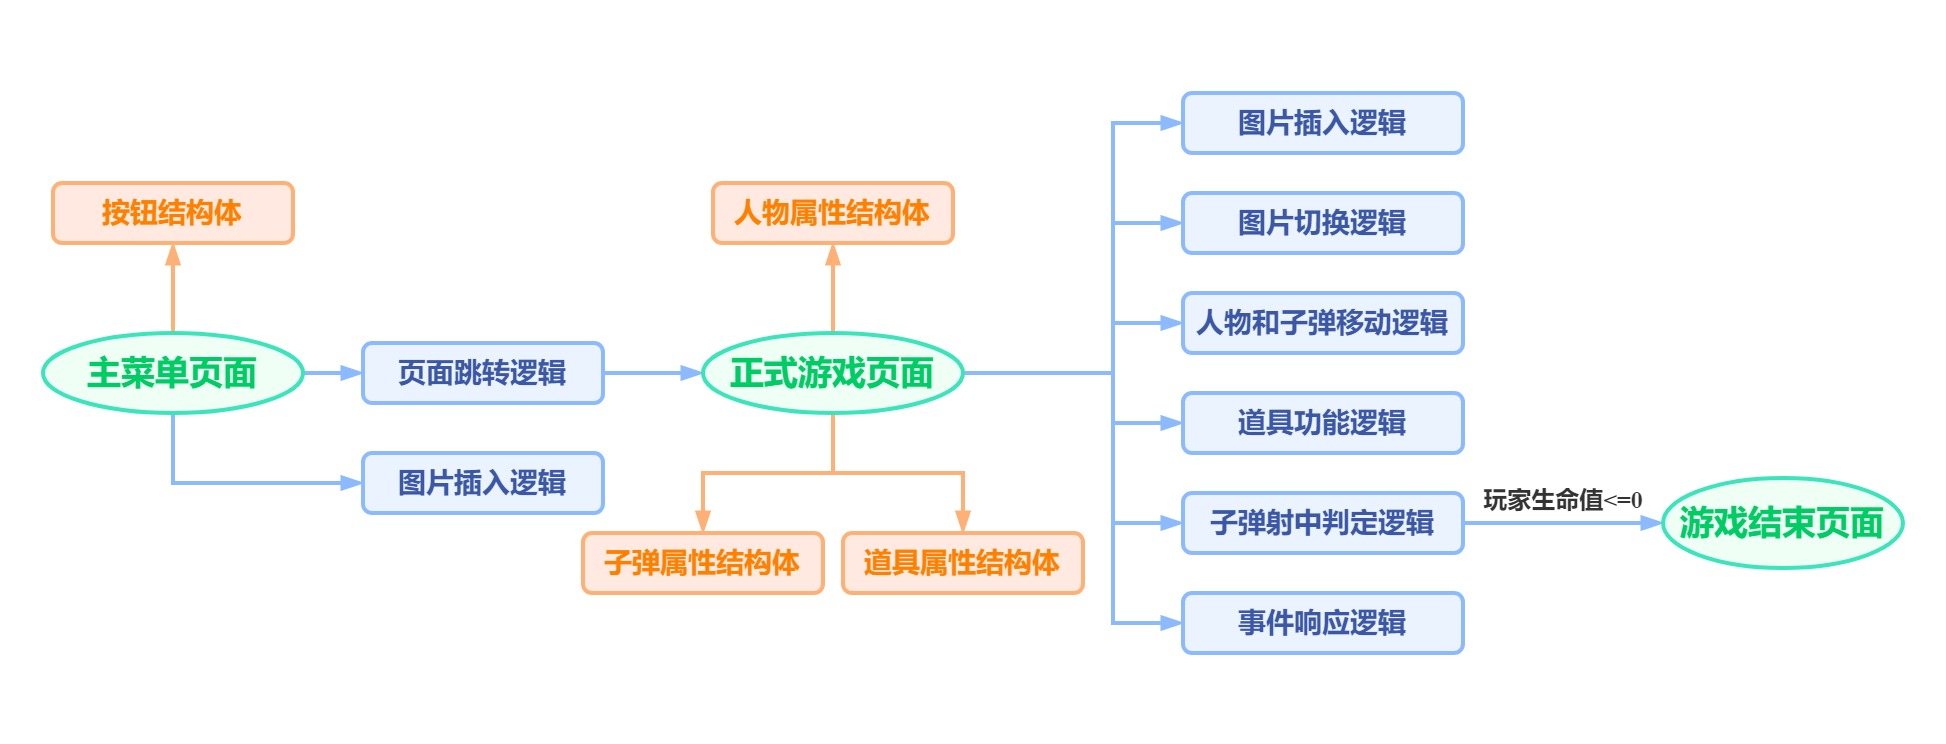
\includegraphics[width=0.8\textwidth]{images/3-1.jpg}
    \caption{游戏逻辑设计分解图}% label 用来在文中索引
\end{figure}
\subsection{页面跳转逻辑}
页面跳转逻辑主要控制游戏中的各种界面的衔接。游戏主要有两个页面,第一个是主菜单页面,第二个是正式游戏页面。主菜单页面作为打开游戏后,玩家能看到的第一个界面,拥有的最主要的功能就是作为一个首界面,实现向正式游戏页面跳转的逻辑。在主菜单页面中,设置两个按钮,一个为“Start”,一个为“Exit”。“Start”按钮在点击后的功能是跳转去“正式游戏页面”。“Exit”按钮在点击后的功能是退出程序运行。
\begin{figure}[htbp]
    \vspace{13pt} % 调整图片与上文的垂直距离
    \
    \centering
    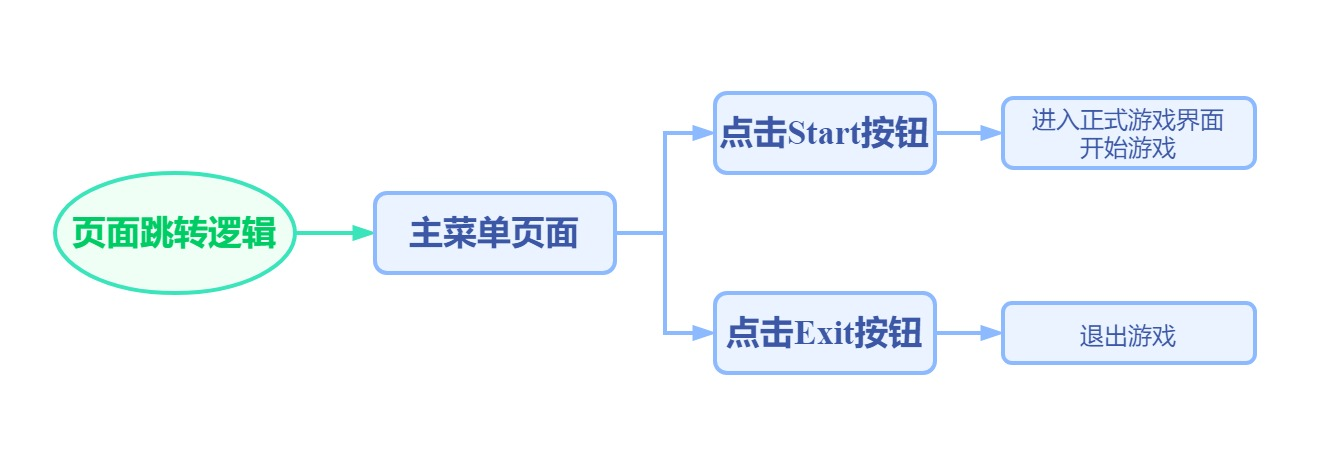
\includegraphics[width=0.8\textwidth]{images/3-2.jpg}
    \caption{页面跳转逻辑示意图}% label 用来在文中索引
\end{figure}
\par
当前界面需要维护的是一个结构体类型MyButton,它的任务是记录当前结构体变量的图片范围——左边界left、右边界right、上边界top、下边界bottom。在具体的代码实现中,定义为start\_button和exit\_button两个结构体变量。
\begin{lstlisting}[language={[x86masm]Assembler}]
    MyButton struct
        top	dd	?
        left	dd	?
        right	dd	?
        bottom	dd	?
    MyButton ends
\end{lstlisting}
\par
页面跳转部分主要依靠全局变量curWindow来控制。在当前页面为主菜单页面时,为curWindow赋值为0;如果当前页面为正式游戏页面,则为curWindow赋值为1。
\subsection{图片插入逻辑和图片切换逻辑}
图片插入逻辑主要控制的是游戏中的界面美观程度和游戏的视觉体验感。在对图片进行制作和处理后,我们确定了所有要插入图片的位置和图片素材,绘制了每个页面的各个图片素材应该出现在的位置的示意草图。
\begin{figure}[htbp]
    \vspace{13pt} % 调整图片与上文的垂直距离
    \centering
    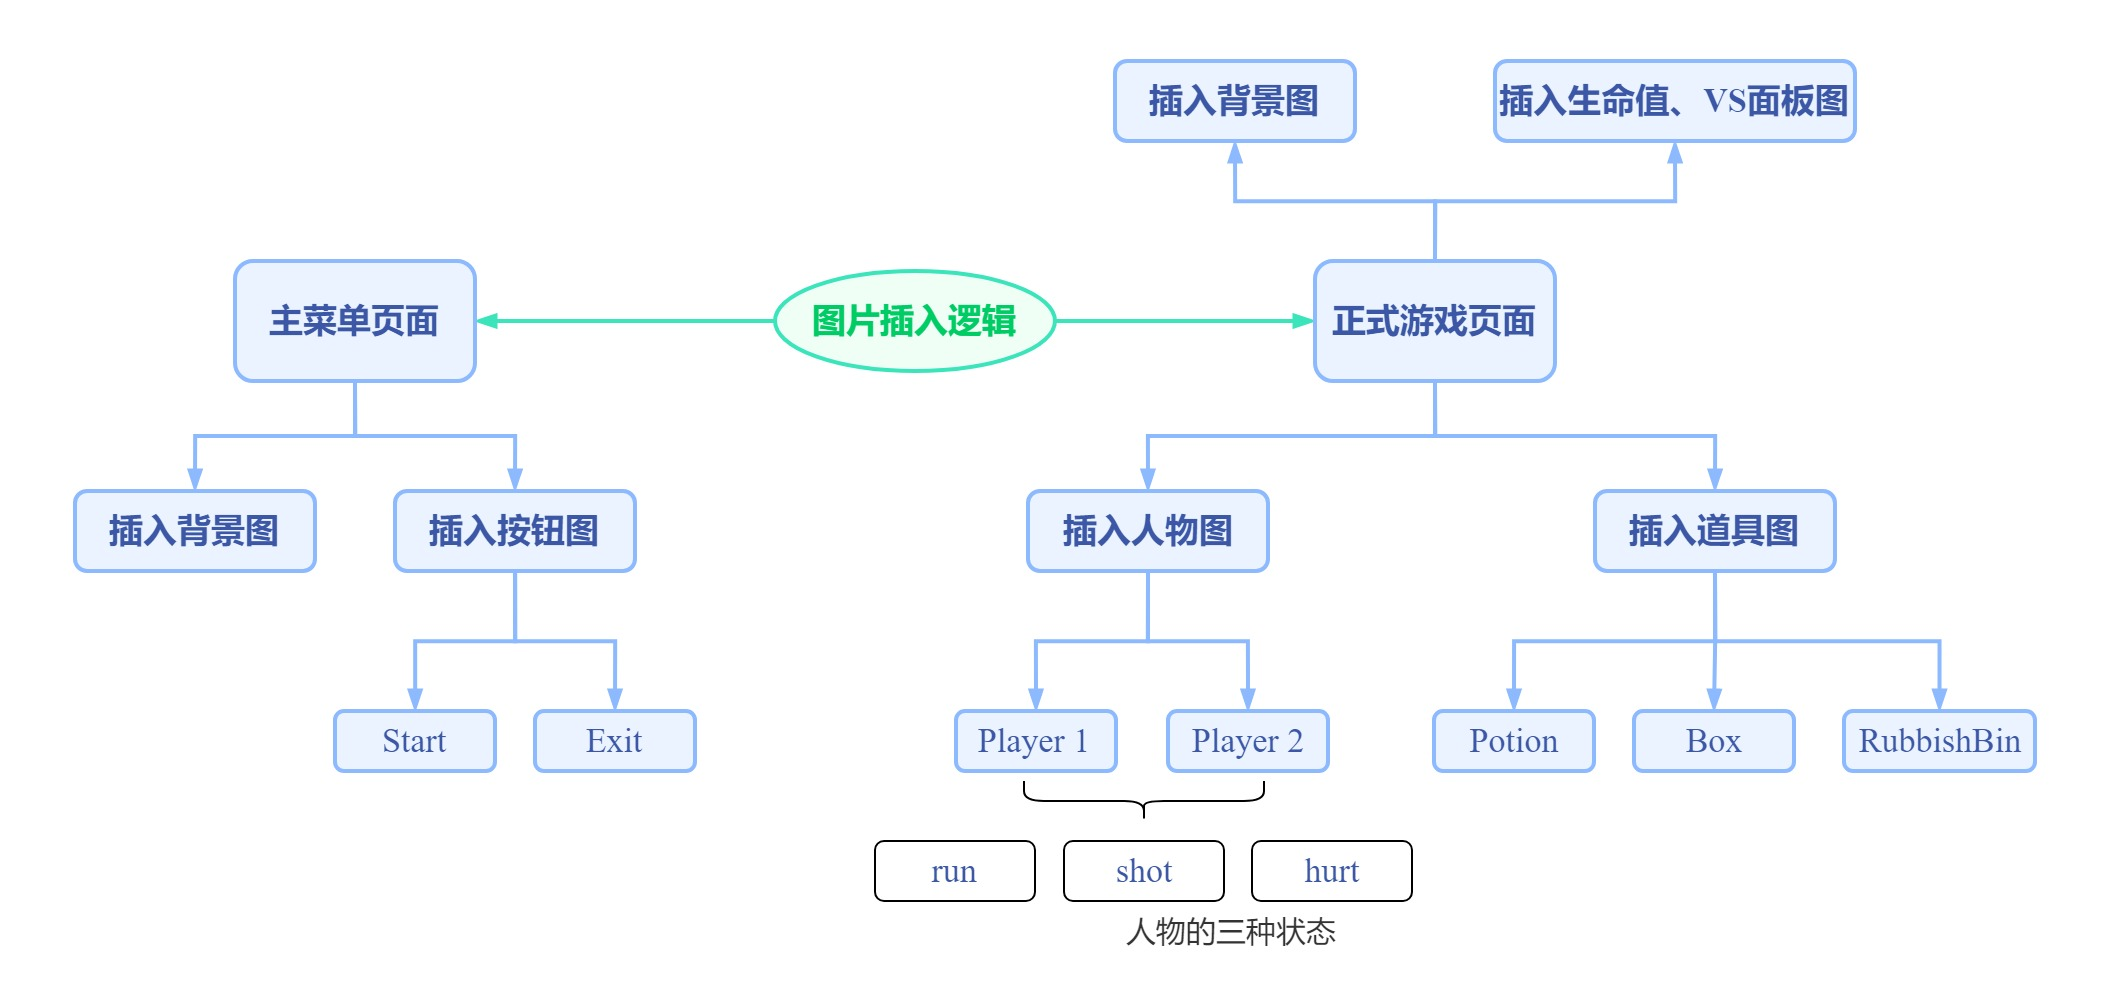
\includegraphics[width=0.7\textwidth]{images/3-3.jpg}
    \caption{图片插入逻辑示意图}% label 用来在文中索引
\end{figure}
\begin{figure}[htbp]
    \vspace{13pt} % 调整图片与上文的垂直距离
    \centering
    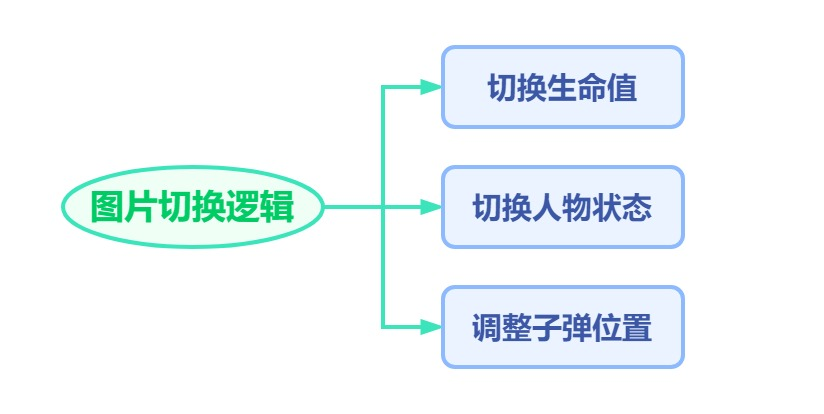
\includegraphics[width=0.5\textwidth]{images/3-4.jpg}
    \caption{图片切换逻辑示意图}% label 用来在文中索引
\end{figure}
\par
我们把图片分为五类,分为按钮、背景、子弹、人物、道具。
\par
主菜单页面只关注主菜单背景图和“Start”、“Exit”按钮图的绘制,因此在start\_menu子程序中,对主菜单页面进行绘制即可,并且在这里加入判断标识curWindow=0,用来表示这是主菜单页面。
\begin{lstlisting}[language={[x86masm]Assembler}]
    start_menu proc C
        ;载入图片
        invoke loadImage, offset page1_Bg, offset imgBg
        invoke loadImage, offset page1_Title, offset imgTitle
        invoke loadImage, offset page1_Start, offset imgStart
        invoke loadImage, offset page1_Exit, offset imgExit	

        ;显示主界面
        invoke beginPaint
        invoke putImageScale, offset imgBg, 0, 0, 800, 600
        invoke putImageScale, offset imgTitle, 200, 100, 400, 100
        invoke putImageScale, offset imgStart, 260, 300, 240, 100
        invoke putImageScale, offset imgExit, 260, 450, 240, 100
        invoke endPaint

        ;设置参数:
        mov curWindow,0
        ret 
    start_menu endp
\end{lstlisting}
\par
接下来,我们调用自己写的draw\_game子程序来实现正式游戏页面的图片绘制、整体图片根据帧数更新位置的功能。正式游戏页面中需要使用到背景、人物、子弹、道具。
\par
在本部分代码的设计过程中,首先我们明确,人物、子弹是同时具有多种属性的。因此我们编写了人物和子弹的结构体,并分别命名为“person”“Bullet”。在整个程序完成编写后,这两个结构体拥有的属性分别如下:
\begin{lstlisting}[language={[x86masm]Assembler}]
    person struct
        life	dd	?;生命值
        pos_x dd ?;横坐标--不变定死
        pos_y dd ?;纵坐标--上下移动
        size_x	dd	?;大小
        size_y	dd	?
        dir	dd	?;移动方向--1为上-1为下
        speed	dd	?;速度大小--
        bullet	dd	?;子弹数
        is_hit dd	?;是否击中或越界
    person ends
    person1 person<>
    person2	person<>

    Bullet struct
        show	dd	?;显示与否
        pos_x dd ?;横坐标
        pos_y dd ?;纵坐标
        dir_x	dd	?;移动方向--1为右,-1为左
        dir_y	dd	?;纵向移动方向 ---用于反弹
        size_x	dd	?;大小
        size_y	dd	?
        speed_x	dd	?;速度大小
        speed_y	dd	?
    Bullet ends
    bullet1 Bullet<>
    bullet2	Bullet<>
\end{lstlisting}
\par
在画背景时,主要使用draw\_bg子程序。该子程序绘制背景、VS图、人物生命值图,并且通过对person结构体中,玩家控制人物的血量进行判断,来决定绘制几个生命值图像(气球)。
\par
在draw\_bg中我们使用ACLLIB提供的库函数loadImage加载图片源;然后使用库函数putImageScale将图片以指定大小展示在前端的指定位置上。而后我们需要根据person结构体的life变量来判定生命值,从而使用条件判断结构在指定位置画出生命值。具体的代码实现如下:
\begin{lstlisting}[language={[x86masm]Assembler}]
    draw_bg proc
        invoke loadImage, offset page2_Bg, offset imgBg2
        invoke loadImage, offset page2_vs, offset imgVS
        ...
        ;分数显示判断
        .if person1.life>=1
            invoke putImageScale, offset imgCharLife1, 145, 495, 30, 50
            .if person1.life>=2
                invoke putImageScale, offset imgCharLife1, 190, 495, 30, 50
                .if person1.life>=3
                    invoke putImageScale, offset imgCharLife1, 235, 495, 30, 50
                    .if person1.life>=4
                        invoke putImageScale, offset imgCharLife1, 280, 495, 30, 50
                        .if person1.life==5
                            invoke putImageScale, offset imgCharLife1, 325, 495, 30, 50
                        .endif
                    .endif
                .endif
            .endif
        ;.elseif person1.life<=0
        ;	invoke game_over
        .endif
        ...
        ret
    draw_bg endp
\end{lstlisting}
\par
在画人物时,首先使用loadImage加载人物的不同状态的图片,然后通过判断person结构体的bullet和is\_hit标志变量来判断人物的形态——如果子弹数为0,则人物当前应该属于“run”的普通行走状态;如果子弹数为1,则人物当前应该属于“shot”的举枪状态。不管人物当前有几颗子弹,只要它中弹,就切换它的贴图为“die”图片。这里的is\_hit的值表示其中弹图片显示的帧数。具体的条件判断实现代码如下:
\begin{lstlisting}[language={[x86masm]Assembler}]
    draw_man proc	
        invoke loadImage, offset page2_char1_run, offset imgCharRun1
        invoke loadImage, offset page2_char2_run, offset imgCharRun2
        ...
        ;通过角色拥有子弹数判断人物形态
        .if person1.bullet==1
            .if person1.is_hit>0;判断中弹
                invoke putImageScale, offset imgCharDie1, person1.pos_x, person1.pos_y,  person1.size_x,  person1.size_y
                sub person1.is_hit,1
            .endif
            .if person1.is_hit==0
                invoke putImageScale, offset imgCharShot1, person1.pos_x, person1.pos_y, person1.size_x,  person1.size_y
            .endif
        .endif
        ...
        ret
    draw_man endp
\end{lstlisting}
\par
在画子弹时,要考虑子弹是在人物举枪以后才能被发射出来,两位玩家操控Player1和Player2,分别使用键盘上的“←”和“→”来控制Player1和Player2的发弹过程,称这两个按键是“发弹键”。子弹的原图是一个直径较小的纯色圆。在人物按下自己对应的发弹键后,人物贴图转换,未触碰道具时,子弹将水平向远离发弹人的方向匀速移动;如果触碰道具,将根据道具的功能来完成子弹的方向调整以及伤害调整。对于子弹结构体中的show属性,当show的值为1时需要画子弹;show的值为0时不需要画子弹。
\begin{lstlisting}[language={[x86masm]Assembler}]
    draw_bullet proc p1:dword,p2:dword
        invoke printf,offset coord,p1,p2
        
        .if p1==1;show为0则不画
            invoke loadImage, offset page2_char1_bul, offset imgCharBul1
            invoke putImageScale, offset imgCharBul1,bullet1.pos_x, bullet1.pos_y, bullet1.size_x, bullet1.size_y
        .endif

        .if p2==1				
            invoke loadImage, offset page2_char2_bul, offset imgCharBul2
            invoke putImageScale, offset imgCharBul2,bullet2.pos_x, bullet2.pos_y, bullet2.size_x, bullet2.size_y			
        .endif
        ret
    draw_bullet endp
\end{lstlisting}
\par
在画道具时,在图片插入逻辑中,关键点在于,要实现道具的随机出现效果。此效果的实现代码放置在draw\_prop子程序、getRand子程序、game\_init子程序、道具属性结构体中。道具属性的结构体主要的目标是记录道具的横纵坐标、大小尺寸。道具分三种,分别拥有变向、增强、降速这三种功能,因此初始化为三类结构体变量Prop\_Bounce、Prop\_Slow、Prop\_Big。
\begin{lstlisting}[language={[x86masm]Assembler}]
    Prop struct
        pos_x dd ?;横坐标
        pos_y dd ?;纵坐标
        size_x	dd	?;大小
        size_y	dd	?
        ;is_hit dd	?;是否击中
    Prop ends
\end{lstlisting}
\par
draw\_prop子程序主要是加载绘制道具图片。getRand子程序用来“随机取数”,在getRand子程序被调用时,参数rand\_num由我们根据想要的个数和图片素材的坐标指定给出,然后随机一个在此范围内的数。game\_init子程序用来“按照随机数放置道具”。在game\_init子程序中,我们依靠时间初始化来随机一个seed,然后调用getRand子程序以达到随机取数的效果,且随机数的范围要小于rand\_num。
\begin{lstlisting}[language={[x86masm]Assembler}]
draw_prop proc
	invoke loadImage, offset page2_box, offset imgObBox
	invoke loadImage, offset page2_rub, offset imgObRubBin
	invoke loadImage, offset page2_potion, offset imgObPotion

	mov ebx,0
	mov edi,0
	.while ebx<Bounce_Num
		invoke putImageScale, offset imgObRubBin,(Prop ptr Prop_Bounce[edi]).pos_x,(Prop ptr Prop_Bounce[edi]).pos_y, (Prop ptr Prop_Bounce[edi]).size_x,(Prop ptr Prop_Bounce[edi]).size_y	
		add edi,type Prop ;Prop大小
		inc ebx
	.endw
    ...
	ret
draw_prop endp
\end{lstlisting}
\subsection{人物和子弹移动逻辑}
子弹和人物的移动实现是通过定时器不断重复调用构成的循环来实现的。每一次循环都被看做一个帧,我们在循环体内更改子弹元素和人物元素的坐标位置并在每个循环中重新绘制,利用人眼的视觉暂留效果,即可实现人物和子弹的动态移动。
\begin{figure}[htbp]
    \vspace{13pt} % 调整图片与上文的垂直距离
    \centering
    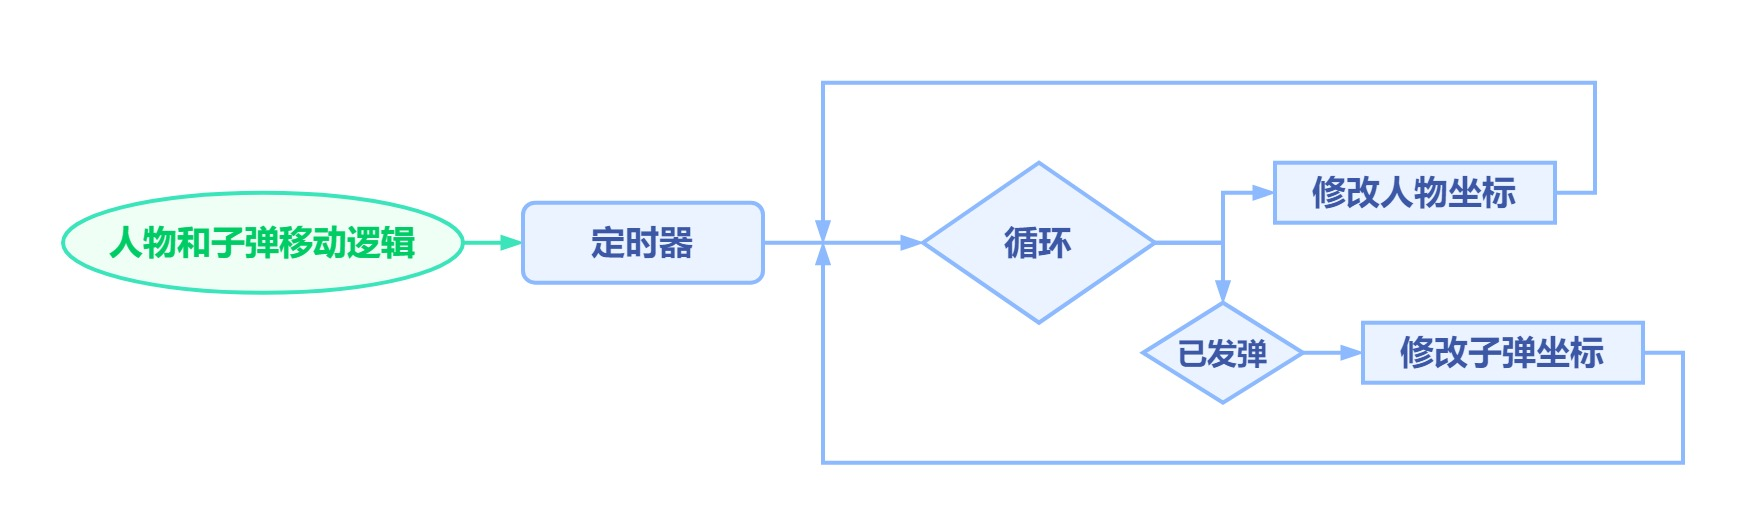
\includegraphics[width=0.8\textwidth]{images/3-5.jpg}
    \caption{人物和子弹移动逻辑示意图}% label 用来在文中索引
\end{figure}
\subsection{道具功能逻辑}
对于两个人物击打道具的判定逻辑都是相同的,只是左边人物的子弹判断的界限是障碍物的左边界,右边人物的子弹判断的界限是障碍物的右边界,所以这里以左边人物为例,介绍击打到不同障碍物时产生的不同效果以及对其的判定逻辑。
\begin{figure}[htbp]
    \vspace{13pt} % 调整图片与上文的垂直距离
    \centering
    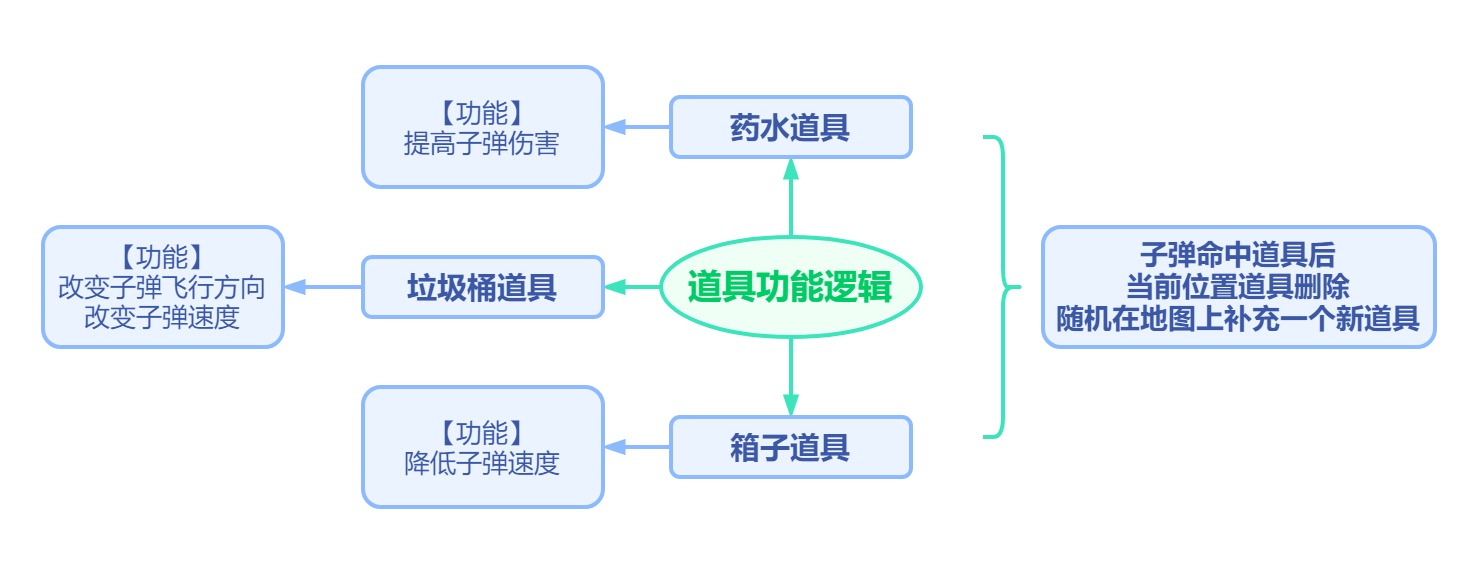
\includegraphics[width=0.8\textwidth]{images/3-6.jpg}
    \caption{道具功能逻辑示意图}% label 用来在文中索引
\end{figure}
\subsubsection{(1)垃圾桶道具}
垃圾桶道具可以实现改变子弹的线路以及速度的功能。对于子弹运行速度的计算,是用x方向的方向标签值乘以x方向的速度,再加上y方向的方向标签值乘以y方向的速度得到的。垃圾桶道具的纵坐标被分为了上中下三个部分,若击打到上半部分,则子弹的y方向标签值设为1,并把此时子弹x方向的速度值直接赋给子弹y方向的速度,从而可以实现子弹以斜向上45度的方向从该道具射出;若击打到中间部分,则子弹的x方向标签值设为-1,即实现了子弹的反弹,子弹有一定概率击打到自己;若击打到下半部分,则子弹的y方向标签值设为-1,并把此时子弹x方向的速度值直接赋给子弹y方向的速度,从而可以实现子弹以斜向下45度的方向从该道具射出。同时垃圾桶道具的功能也支持叠加,从而实现了子弹方向与速度的不断变换。
\begin{lstlisting}[language={[x86masm]Assembler}]
    .if edx>=bound_left && edx<=bound_right	&& ebx<=bound_up &&  ebx>=bound_down;x在范围内						
            .if ebx>=bound_m_up && ebx<=bound_up;上半部 ;speed_y+=speed_x dir_y=1
                mov bullet1.dir_y,1
                mov eax,bullet1.speed_x
                add eax,bullet1.speed_y
                mov bullet1.speed_y,eax
            .endif
            .if ebx>=bound_m_down && ebx<=bound_m_up;中间反弹 dir_x反向
                mov eax,-1
                imul bullet1.dir_x
                mov bullet1.dir_x,eax
            .endif
            .if ebx<=bound_m_down && ebx>=bound_down	;下面反弹
                mov bullet1.dir_y,-1
                mov eax,bullet1.speed_x
                add eax,bullet1.speed_y
                mov bullet1.speed_y,eax
            .endif		
            ;重新更新位置
            invoke getRand,370;150-600为人物x坐标
            add eax,190;范围 190-560
            mov (Prop ptr Prop_Bounce[edi]).pos_x,eax

            invoke getRand,200;160-400为人物上下界
            add eax,180;范围 180-580
            mov (Prop ptr Prop_Bounce[edi]).pos_y,eax
            ;invoke printf,offset coord,eax,eax			
    .endif
\end{lstlisting}
\subsubsection{(2)箱子道具}
箱子道具可以实现子弹的慢速。当子弹射中箱子道具时,子弹x方向的速度值会减4,且该效果可以叠加。为了防止子弹速度减为0,当速度值减小到0以下后,会被设置为速度的最低阈值。
\begin{lstlisting}[language={[x86masm]Assembler}]
    .if edx>=bound_left && edx<=bound_right	&& ebx<=bound_up &&  ebx>=bound_down;x在范围内								
            sub bullet1.speed_x,4
            .if bullet1.speed_x <= 0
                mov bullet1.speed_x,2
            .endif

            ;重新更新位置
            invoke getRand,370;150-600为人物x坐标
            add eax,190;范围 190-560
            mov (Prop ptr Prop_Slow[edi]).pos_x,eax

            invoke getRand,200;160-400为人物上下界
            add eax,180;范围 180-580
            mov (Prop ptr Prop_Slow[edi]).pos_y,eax
            ;invoke printf,offset coord,eax,eax			
    .endif
\end{lstlisting}
\subsubsection{(3)药水道具}
药水道具可以实现子弹的威力增强。普通子弹会对人物造成一滴血的伤害,但若子弹在运行过程中碰到了药水道具,则子弹功能增强,当打到人物时会造成两滴血的伤害,且药水道具的作用可以叠加。如果子弹射中了药水道具,则此时击打到药水道具的标志值就会加1。如果该子弹击中了人物,则人物血量的变化会根据该标志值改变,如果标记值为0,则人物血量减1;如果标记值大于0,则每次人物血量减2,标志值减1,循环直至标记值为0,人物血量判定结束。
\begin{lstlisting}[language={[x86masm]Assembler}]
    .if edx>=bound_left && edx<=bound_right	&& ebx<=bound_up &&  ebx>=bound_down;x在范围内								
            inc	Big_flag1
            ;重新更新位置
            invoke getRand,370;150-600为人物x坐标
            add eax,190;范围 190-560
            mov (Prop ptr Prop_Big[edi]).pos_x,eax

            invoke getRand,200;160-400为人物上下界
            add eax,180;范围 180-580
            mov (Prop ptr Prop_Big[edi]).pos_y,eax
            ;invoke printf,offset coord,eax,eax			
    .endif
\end{lstlisting}
\par
当子弹射击到任意一个道具后,该道具都会消失,然后会再产生随机数,确定更新道具的位置,消失道具与更新道具的类型是相同的。
\subsection{子弹射中判定逻辑}
\begin{figure}[htbp]
    \vspace{13pt} % 调整图片与上文的垂直距离
    \centering
    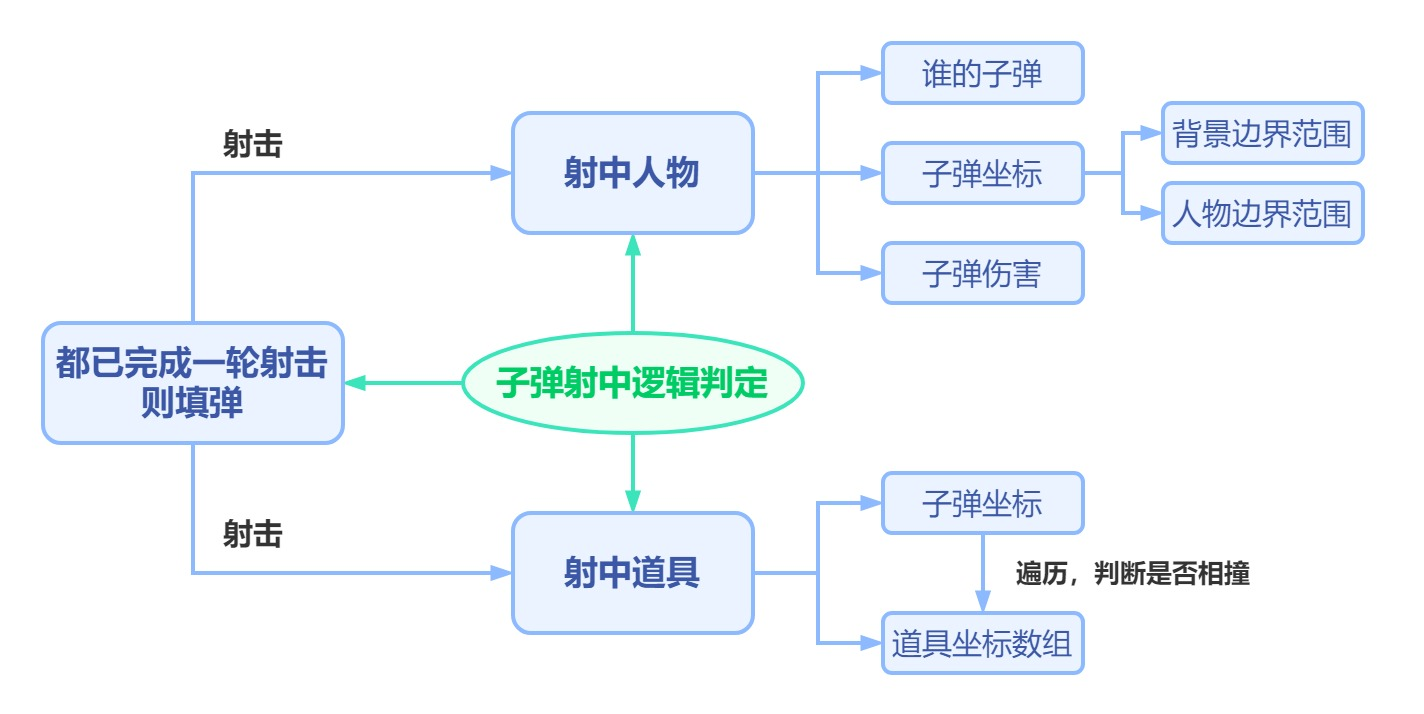
\includegraphics[width=0.7\textwidth]{images/3-7.jpg}
    \caption{子弹射中判定逻辑}% label 用来在文中索引
\end{figure}
\par
\subsubsection{(1)子弹射中人物判定}
根据游戏机制,人物只能由对方的子弹射中。所以我们在设计check\_hit\_person子程序的时候传入了三个参数,分别是子弹的x,y坐标和子弹的归属。对于已发射的子弹而言,我们需要判断子弹的位置是否与人物位置重合,若重合则判定中弹。在中弹的逻辑内我们将person2.is\_hit标志变量设为10,表示人物中弹的状态显示10帧。然后判断子弹是否为加强弹,根据这个更改子弹的伤害值。
\begin{lstlisting}[language={[x86masm]Assembler}]
	.if p==1
	mov eax,person2.pos_y
	sub eax,30
	mov bound_down,eax
	add eax,60
	mov bound_up,eax
	mov eax,person2.pos_x
	sub eax,30
	mov bound_left,eax
	add eax,60
	mov bound_right,eax
	.if ecx<=bound_right && ecx>=bound_left && ebx <= bound_up && ebx >=bound_down
			mov person2.is_hit,10;为了让中弹的样子显示更清楚些,显示10帧
				invoke printf,offset coord,111 ,Big_flag1
				.if  Big_flag1 !=0
					.while Big_flag1>0
						sub person2.life,2
						dec Big_flag1
						invoke printf,offset life2Test,person2.life
					.endw
				.else 
					sub person2.life,1
					invoke printf,offset life2Test,person2.life
				.endif
			.if person2.life == Zero || person2.life == -1 || person2.life == -2 ||person2.life == -3 || person2.life == -4 || person2.life == -5 ||person2.life == -6 ||person2.life == -7 ||person2.life == -8 ||person2.life == -9 ||person2.life == -10
				invoke printf,offset tip,person2.life
				mov person2.life,0
				;invoke game_over
			.endif 
			;填弹逻辑代码在下面展示
            ...
	.endif
	.endif
\end{lstlisting}
\par
对于子弹射出边界,我们根据位置判定若为上下界则反弹,若为左右界则消失。具体的代码实现如下:
\begin{lstlisting}[language={[x86masm]Assembler}]
	.if ecx>= 800 || ecx<=0
		mov bullet1.show,0
		.if person2.bullet == 0 && bullet1.show == 0 && bullet2.show == 0
			mov person1.bullet,1
			mov person2.bullet,1
		.endif
	.endif
	.if (ebx >400 || ebx <160)
			mov eax,-1
			imul bullet1.dir_y
			mov bullet1.dir_y,eax
	.endif
\end{lstlisting}
\par
在射击完子弹后,我们需要判定是否需要填弹,具体的实现逻辑是若玩家1的子弹完成作用时玩家2的子弹夹为0,则两者全部填弹;反之则不做操作。具体的代码实现如下:
\begin{lstlisting}[language={[x86masm]Assembler}]
    mov bullet1.show,0
    .if person2.bullet == 0 && bullet1.show == 0 && bullet2.show == 0
        mov person1.bullet,1
        mov person2.bullet,1
    .endif
\end{lstlisting}
\subsubsection{(2)子弹射中道具判定}
\par
对于子弹射中道具,我们需要获取到子弹的位置,然后去遍历道具数组来判定是否与道具位置相撞。若相撞则根据道具功能来对子弹加以相关特性。这里的判定逻辑不做赘述。遍历道具数组的代码实现如下:
\begin{lstlisting}[language={[x86masm]Assembler}]	
	local bound_up:dword	;up-m_up子弹向上弹
	local bound_m_up:dword	;m_up-m_down 反弹
	local bound_m_down:dword;m_down-down 向下弹
	local bound_down:dword

	local bound_left:dword
	local bound_right:dword
	.if p==1;1发的子弹
		;edx循环计数,ecx,ebx xy坐标
		mov edi,0
		mov ecx,0
		mov ebx,y
		mov edx,x
		;Bounce
		.while ecx<Bounce_Num
			;道具效果已展示,不再赘述
			...
			add edi,type Prop ;Prop大小
			inc ecx	
		.endw
\end{lstlisting}
\subsection{事件响应逻辑}
\begin{figure}[htbp]
    \vspace{13pt} % 调整图片与上文的垂直距离
    \centering
    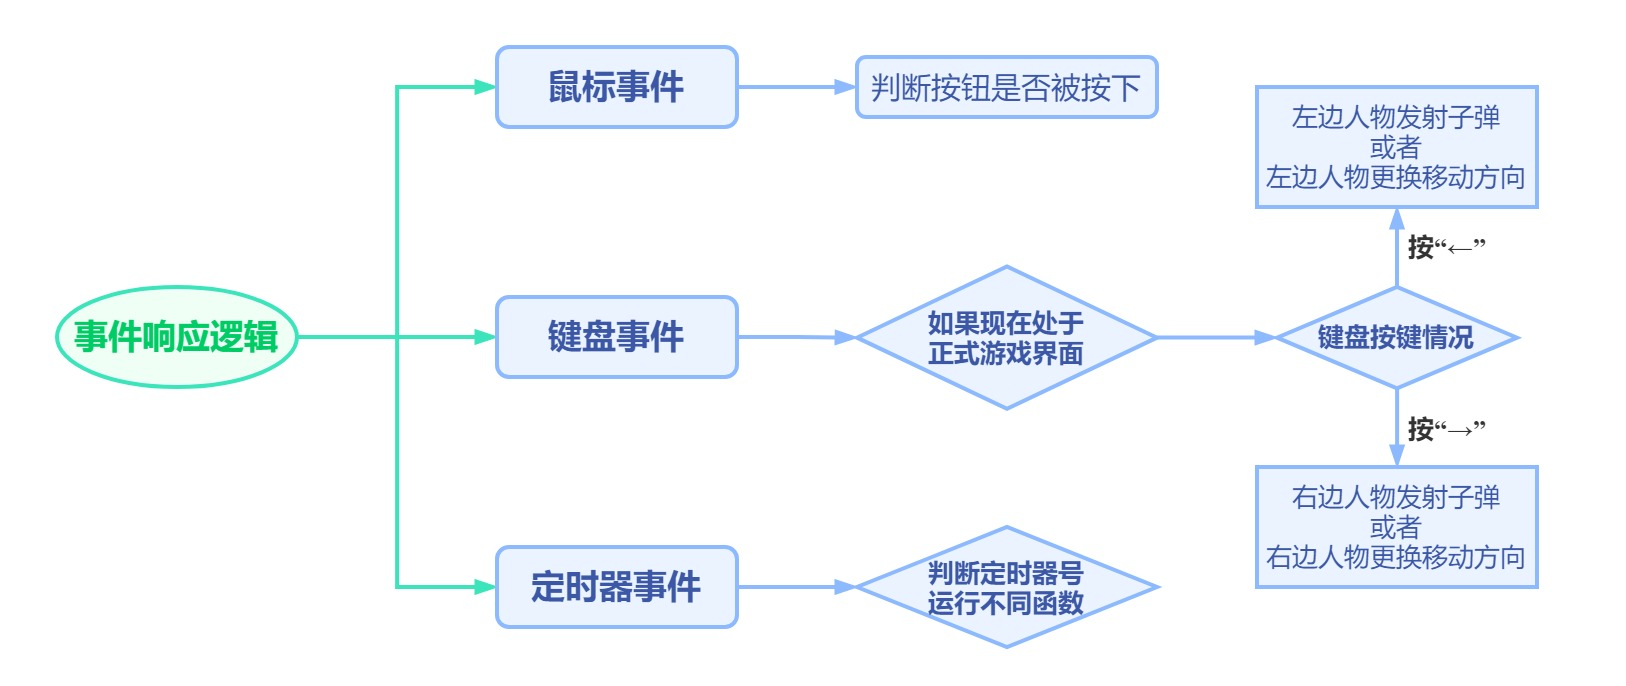
\includegraphics[width=0.8\textwidth]{images/3-8.jpg}
    \caption{事件响应逻辑示意图}% label 用来在文中索引
\end{figure}
\subsubsection{(1)鼠标事件}
单击按钮时,需要判断出当前有鼠标点击,且鼠标点击的位置是否为按钮图片所在的范围。因此使用iface\_mouseEvent和judge\_area子程序来完成按钮的点击效果,实现页面跳转。子程序iface\_mouseEvent是用来判断鼠标是否进行了点击操作的。如果鼠标左键按下,则调用judge\_area子程序对鼠标的点击范围进行判断;在judge\_area子程序中,通过对比start\_button中的范围(即“Start”的范围)和鼠标的坐标大小关系,来确定鼠标坐标是否在“Start”的图片范围之内,如果在的话,就给eax寄存器存值1,否则存0。回归iface\_mouseEvent判断分支,判断eax的值,如果eax为1,说明玩家已经按下“Start”,则通过game\_init子程序完成正式游戏界面的绘制。并且打开定时器0,并以30ms的时间间隔调用计时器0中的函数,实现游戏界面中基本循环的运行。
\begin{lstlisting}[language={[x86masm]Assembler}]
    iface_mouseEvent proc C x:dword,y:dword,button:dword,event:dword
        .if button == LEFT_BUTTON && event == BUTTON_DOWN
            .if	curWindow == 0;当前在主界面
                invoke judge_area,x,y,start_button.left,start_button.right,start_button.top,start_button.bottom
                .if eax==1
                    invoke printf,offset coord,x,y
                    ;游戏开始,设置初始值
                    invoke game_init
                    ;开启循环,30ms触发
                    invoke startTimer,0,30
                .endif
                invoke judge_area,x,y,exit_button.left,exit_button.right,exit_button.top,exit_button.bottom
                .if eax ==1
                    invoke ExitProcess, NULL
                .endif

            .endif
            .if curWindow == 2
                invoke judge_area,x,y,exit_button.left,exit_button.right,exit_button.top,exit_button.bottom
                .if eax ==1
                    invoke ExitProcess, NULL
                .endif
            .endif
        .endif
        ret
    iface_mouseEvent endp
    judge_area proc C uses ebx x:dword,y:dword,left:dword,right:dword,top:dword,bottom:dword
        ;x,y为鼠标按下位置
        mov eax,x
        mov ebx,y
        .if	eax <= left || eax >=right || ebx >= bottom || ebx <= top
            mov eax,0
        .else	
            mov eax,1
        .endif	
        ret
    judge_area endp
\end{lstlisting}
\par
如果在判断鼠标范围时发现鼠标并未在“Start”的范围中点击,则进入“判断是否为‘Exit’按钮”分支。调用judge\_area子程序,通过对比exit\_button中的范围(即”Exit“的范围)和鼠标的坐标大小关系,来确定鼠标是否在“Exit”的范围之内,如果在的话eax此时会变为1,通过判断eax等于1,来决定调用退出进程的子程序。
\subsubsection{(2)键盘事件}
如果当前curWindow为1,即代表是游戏界面,则根据键盘的输入来决定接下来的操作。在该游戏中,键盘总共会有两个输入,即“←”“→”,分别代表左边人物发射子弹和右边人物发射子弹。当判断键盘输入为“←”,且该按键被按下时,首先判断当前人物(即左边人物)是否拥有子弹,如果没有子弹,则更换其运行的方向,不能进行射击行为;如果当前有子弹,则子弹清0,得到当前人物的位置,该位置即为子弹开始显示的坐标,并给子弹设置向右运行的方向标志(即x方向为1,y方向为0),以及子弹每个方向上的速度(即x方向和y方向)。对于子弹运行速度的计算,是用x方向的方向标签值乘以x方向的速度,再加上y方向的方向标签值乘以y方向的速度。最后再把子弹可以显示的标志设为1,确保子弹的正确显示。
\begin{lstlisting}[language={[x86masm]Assembler}]
    iface_keyboardEvent proc C key:dword,event:dword
        .if curWindow == 1
            ;invoke printf,offset coord,person1.dir,person2.dir
            .if key == VK_LEFT && event==BUTTON_DOWN;按下左键,!!注意一定要是按下;不然算两次
                .if person1.bullet==1;有子弹
                    mov person1.bullet,0
                    ;其他子弹操作:设置子弹初始化信息
                    mov eax,person1.pos_x
                    mov bullet1.pos_x,eax
                    mov eax,person1.pos_y
                    mov bullet1.pos_y,eax
                    mov bullet1.dir_x,1
                    mov bullet1.dir_y,0
                    mov bullet1.speed_x,12
                    mov bullet1.speed_y,12
                    mov bullet1.show,1
                .else ;换方向
                    mov eax,-1
                    imul person1.dir
                    mov person1.dir,eax
                .endif
            .endif
            ...
        .endif
        ret
    iface_keyboardEvent endp
\end{lstlisting}
\subsubsection{(3)定时器事件}
注册了定时器事件后,便会根据定时器号选择运行不同的函数。在该游戏中,即当定时器号为0时,则会调用draw\_game的函数,开始游戏界面的绘制。并且根据打开定时器0时对应函数语句的设置,每隔30ms就会调用一次该定时器事件。
\begin{lstlisting}[language={[x86masm]Assembler}]
    iface_timerEvent proc c tid: dword
        .if tid == 0;游戏主循环
            invoke draw/_game
        .endif
        ret
    iface_timerEvent endp
\end{lstlisting}
\section{技术亮点}
在本游戏项目中,我们的程序拥有以下技术亮点:
\begin{itemize}
    \item 使用随机位置算法:我们通过自定义一个seed来在getRand中更新生成的随机数,然后用于位置的坐标中,实现位置的随机化。
    \item 道具的功能多样化,分别具有改变子弹飞行方向、改变子弹速度、改变子弹伤害等效果,这些效果的算法由我们自己编写及实现。
    \item 实现动画效果:通过人眼视觉暂留的原理,对图片的坐标位置和切换逻辑按帧进行规定,使其按帧发生变化,从而人眼获取到的就是动态的动画效果。
    \item 按钮判定:我们没有采用一般的窗口编程的按钮实现和点击事件判定方法,而是通过制作一个按钮的图片,然后判定图片的范围和鼠标单击位置的坐标,如果位置在图片上,则说明点到了此按钮,进入按钮点击后的对应逻辑。
    \item 自定义图片和音乐:本游戏的部分图片素材由我们根据《Among us》游戏的素材自己二次制作而成,另一部分图片素材由我们自己使用Photoshop制作,图片和音乐的风格都符合游戏的风格特色。
\end{itemize}


\chapter{玩家手册}
\section{运行和卸载方式}
针对我们的游戏,有两种方式可以运行:如果使用VS运行项目,则直接删除项目即可删除游戏;如果使用我们给出的安装程序运行项目,则需要使用安装程序卸载项目。
\subsection{使用VS运行项目}
在依照“第2章 开发环境”中的MSVC工具集版本、并选择好当前项目的配置环境(如masm32库的位置链接等)后,使用VS打开本实验项目,选择上方调试-开始执行(不调试)运行项目。
\subsection{使用安装程序运行项目}
我们使用VS自带的Setup扩展内容完成了整体项目的打包发布。打包后的压缩包名称为“Debug.zip”,解压该文件后,会生成以下文件:setup.exe可以完成项目软件的安装;.msi文件可以完成对软件的卸载以及修复。
\begin{figure}[htbp]
    \vspace{13pt} % 调整图片与上文的垂直距离
    \centering
    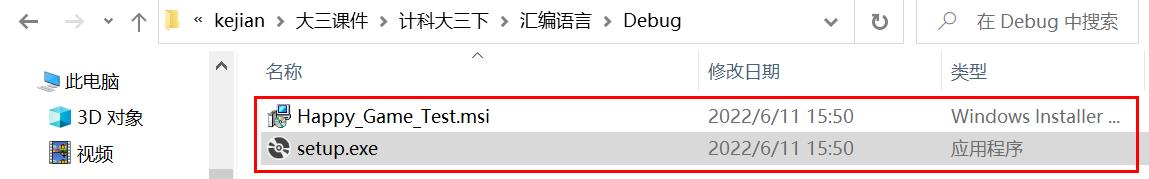
\includegraphics[width=0.8\textwidth]{images/4-1.jpg}
    \caption{解压以后的文件}% label 用来在文中索引
\end{figure}
\par
双击setup.exe,会弹出图4-2,单击“下一步”:
\par
\begin{figure}[htbp]
    \vspace{13pt} % 调整图片与上文的垂直距离
    \centering
    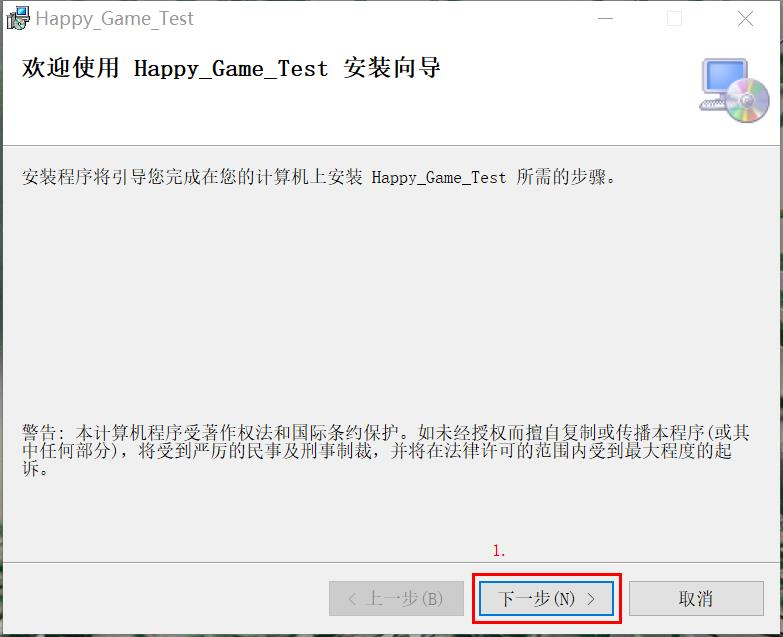
\includegraphics[width=0.5\textwidth]{images/4-2.jpg}
    \caption{安装页面}% label 用来在文中索引
\end{figure}
\par
自定义程序所在文件夹,选择“任何人”,单击“下一步”。
\par
\begin{figure}[htbp]
    \vspace{13pt} % 调整图片与上文的垂直距离
    \centering
    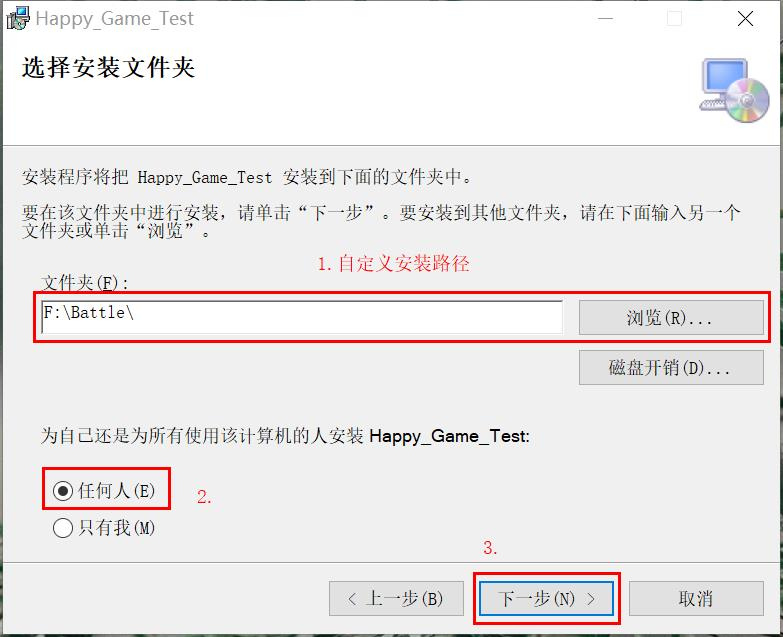
\includegraphics[width=0.5\textwidth]{images/4-3.jpg}
    \caption{选择安装路径页面}% label 用来在文中索引
\end{figure}
\par
单击“下一步”,进行安装。
\par
\begin{figure}[htbp]
    \vspace{13pt} % 调整图片与上文的垂直距离
    \centering
    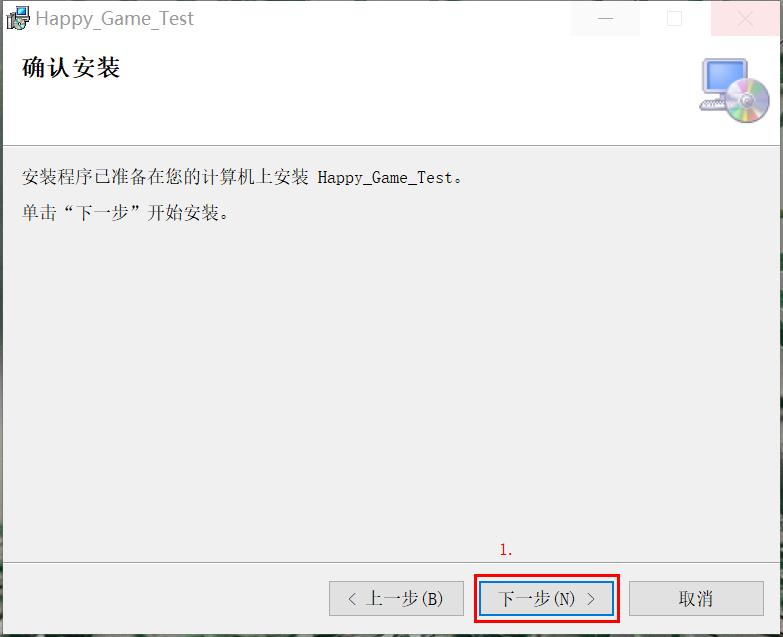
\includegraphics[width=0.5\textwidth]{images/4-4.jpg}
    \caption{确认安装}% label 用来在文中索引
\end{figure}
\par
完成安装。
\par
\begin{figure}[htbp]
    \vspace{13pt} % 调整图片与上文的垂直距离
    \centering
    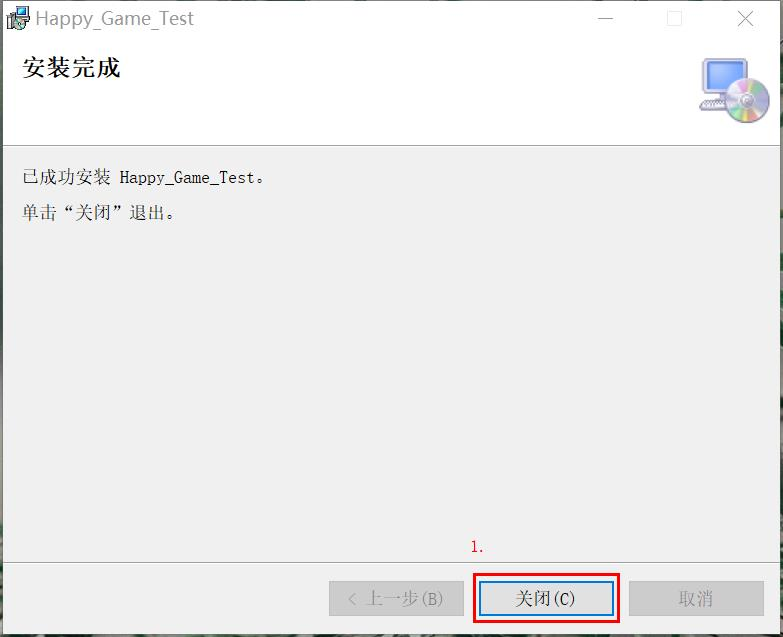
\includegraphics[width=0.5\textwidth]{images/4-5.jpg}
    \caption{安装完成}% label 用来在文中索引
\end{figure}
\par
在图4-3中自定义的文件路径里,可以找到以下文件:
\par
\begin{figure}[htbp]
    \vspace{13pt} % 调整图片与上文的垂直距离
    \centering
    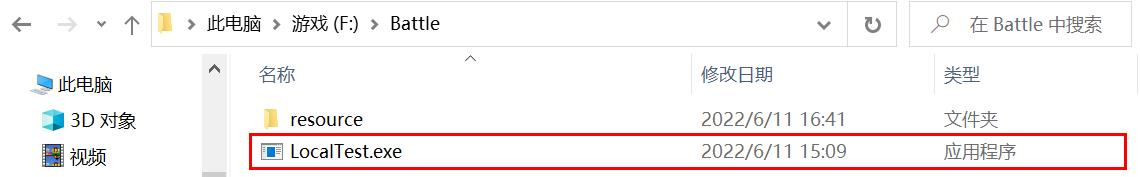
\includegraphics[width=0.8\textwidth]{images/4-6.jpg}
    \caption{生成的可执行文件}% label 用来在文中索引
\end{figure}
\par
双击“LocalTest.exe”后即可运行。
\par
在完成安装后,桌面还会生成一个快捷方式,双击快捷方式也可以直接运行游戏。
\par
\begin{figure}[htbp]
    \vspace{13pt} % 调整图片与上文的垂直距离
    \centering
    
\includegraphics[]{images/4-7.jpg}
    \caption{快捷方式}% label 用来在文中索引
\end{figure}
\subsection{使用安装程序卸载游戏}
在图4-1中,双击“.msi”格式结尾的文件,弹出图4-8。
\par
选中“删除Happy\_Game\_Test(M)”,然后单击“完成”。
\par
\begin{figure}[htbp]
    \vspace{13pt} % 调整图片与上文的垂直距离
    \centering
    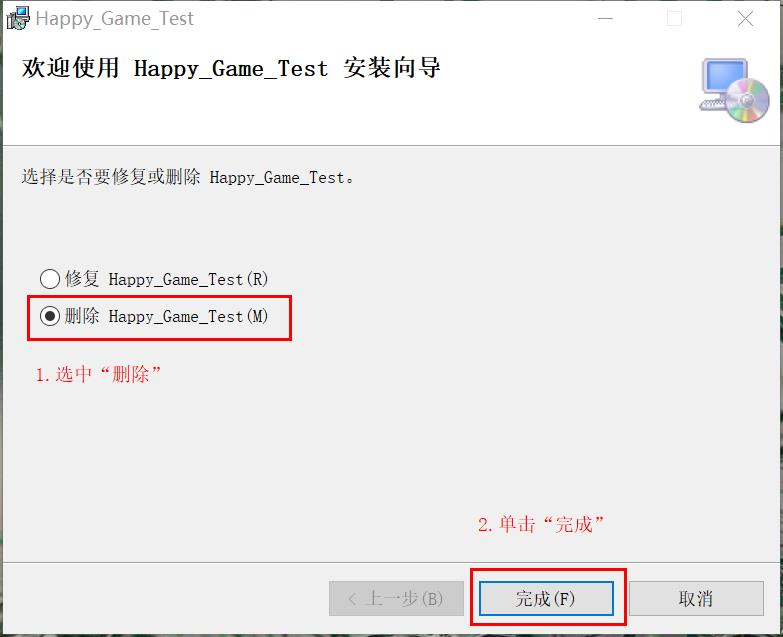
\includegraphics[]{images/4-8.jpg}
    \caption{使用安装程序删除本地已安装游戏}% label 用来在文中索引
\end{figure}
\par
在删除成功之后,单击“关闭”关闭窗口就完成了整个删除流程。
\par
\begin{figure}[htbp]
    \vspace{13pt} % 调整图片与上文的垂直距离
    \centering
    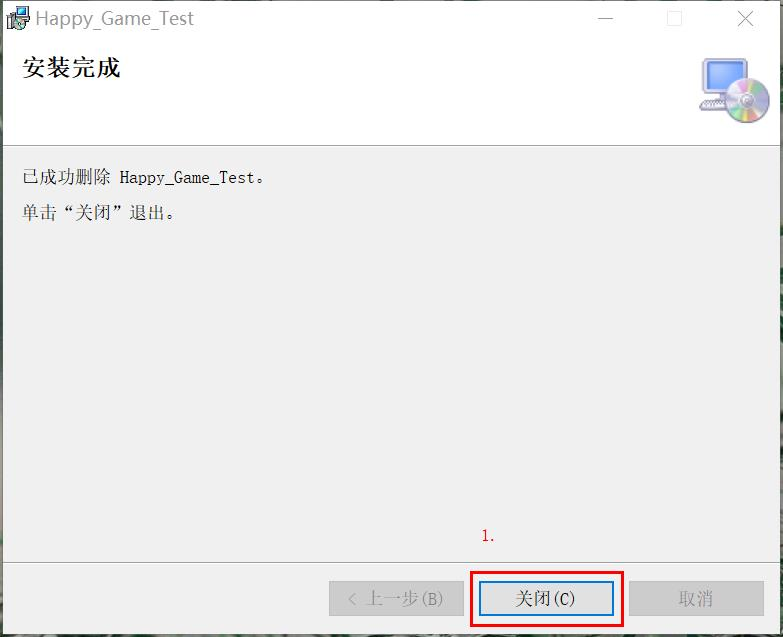
\includegraphics[]{images/4-9.jpg}
    \caption{删除成功}% label 用来在文中索引
\end{figure}
\section{运行效果与功能说明}
进入游戏后我们可以看到游戏的开始界面,其中包括Strat和Exit两个选项;点击Start我们就进入了正式游戏页面,点击Exit则会退出程序运行,关闭游戏。
\par
\begin{figure}[htbp]
    \vspace{13pt} % 调整图片与上文的垂直距离
    \centering
    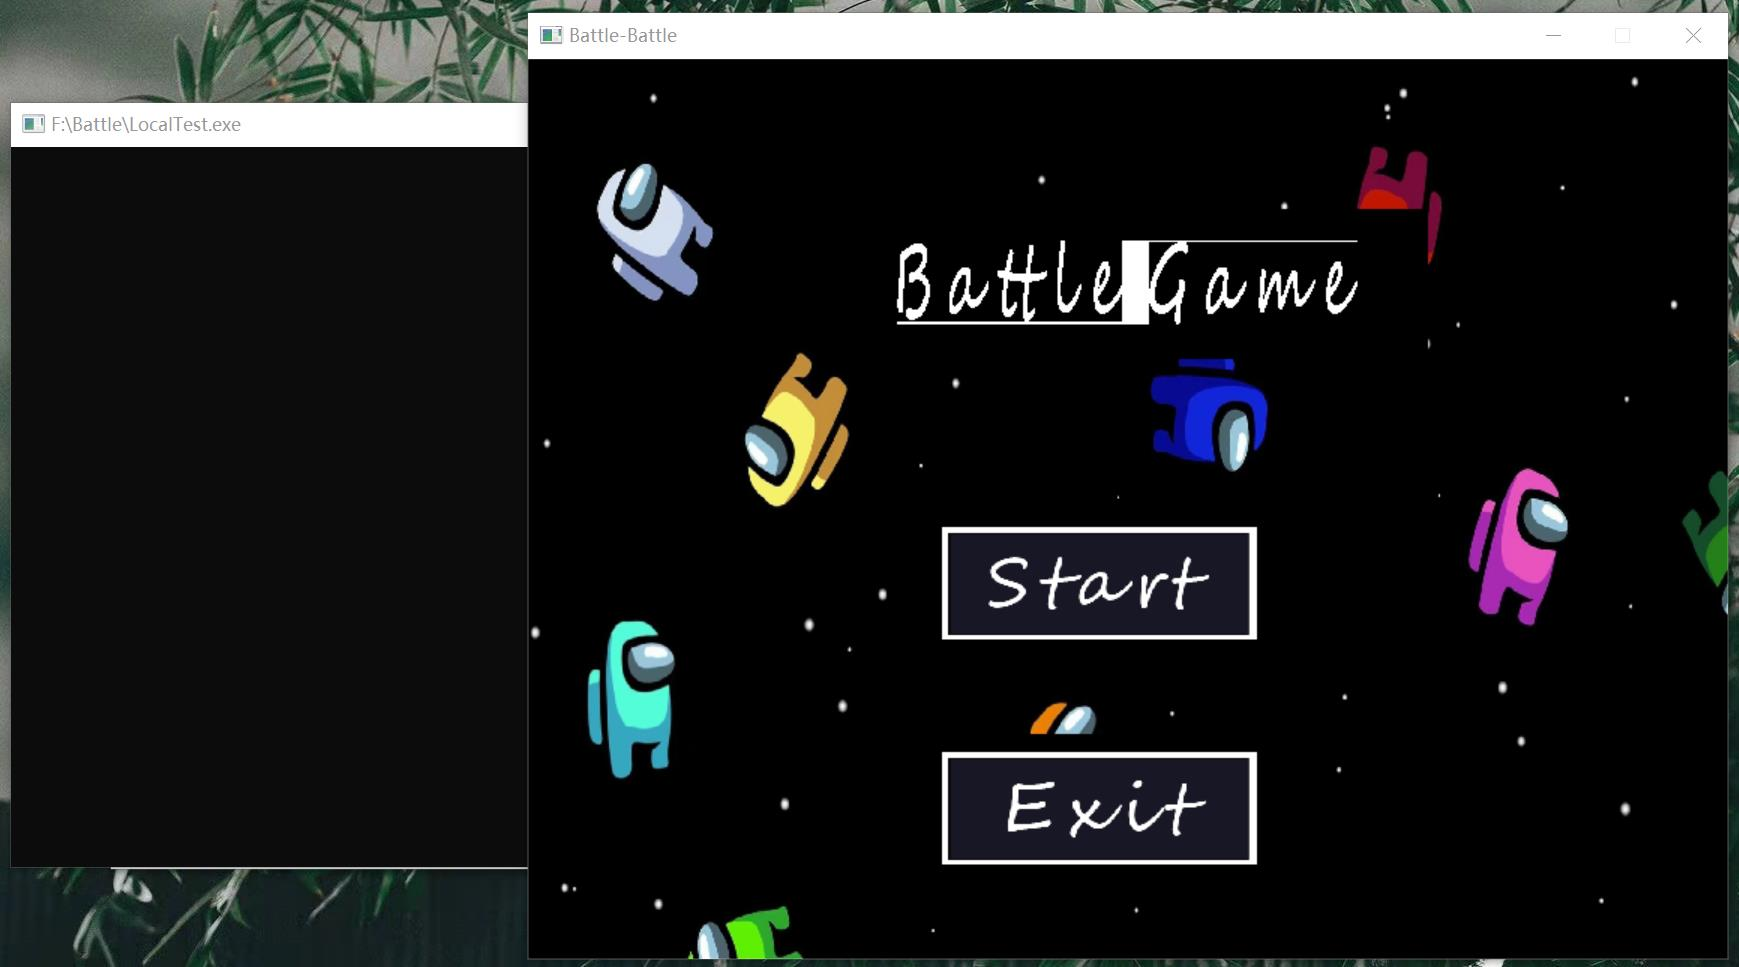
\includegraphics[width=0.8\textwidth]{images/4-10.jpg}
    \caption{游戏主菜单界面}% label 用来在文中索引
\end{figure}
\par
在游戏页面我们可以看到左右两边有两个自己移动的人物,此时游戏已经开始。游戏底部“VS”板上显示的气球代表两个玩家操作人物的生命值,在人物被击中之后生命值会依据子弹的伤害减少对应的值。
\par
\begin{figure}[htbp]
    \vspace{13pt} % 调整图片与上文的垂直距离
    \centering
    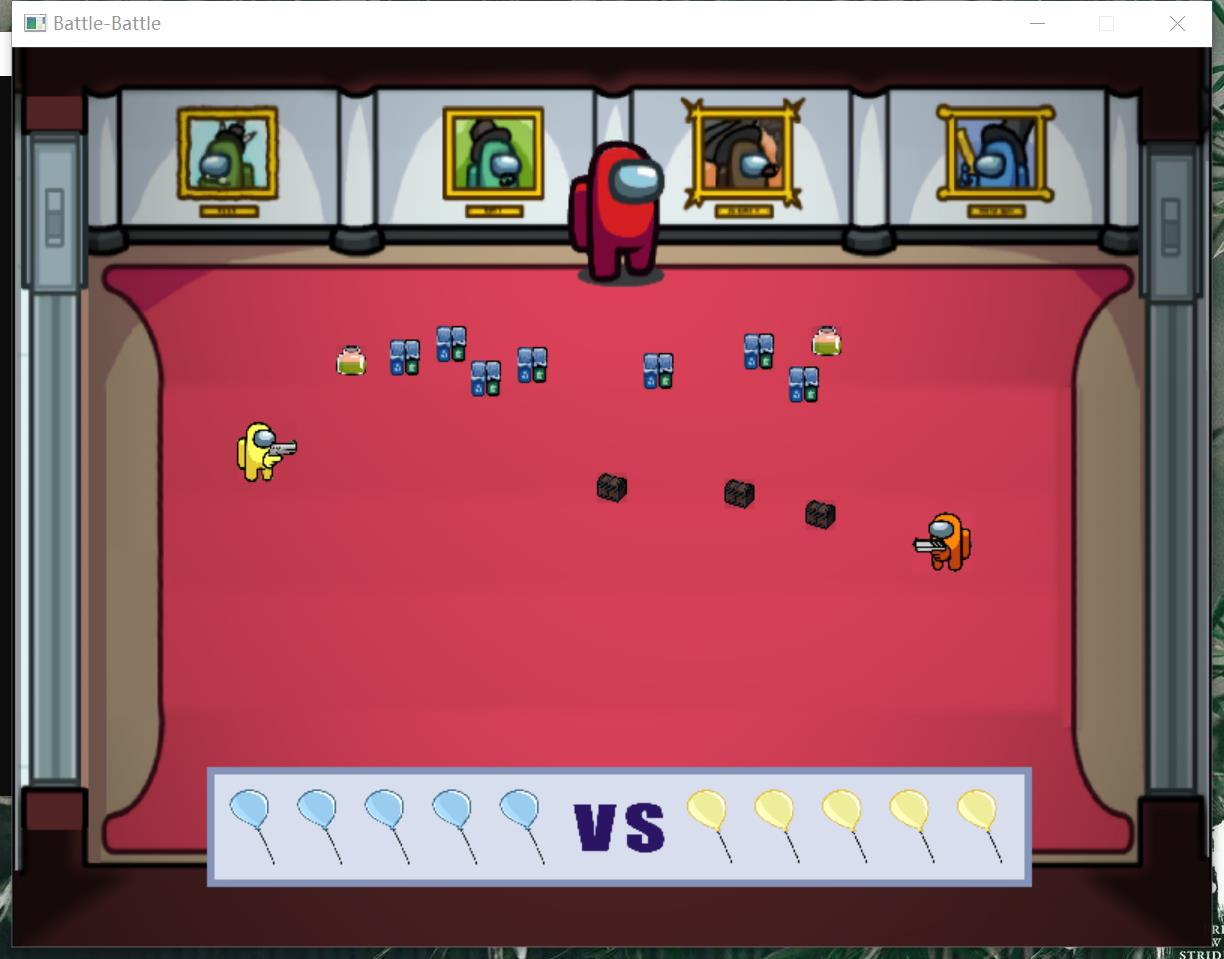
\includegraphics[width=0.8\textwidth]{images/4-11.jpg}
    \caption{正式游戏界面}% label 用来在文中索引
\end{figure}
\par
操作方式:按下键盘上的“⬅”可以让左边的人物发弹/改变移动方向;按下键盘上的“→”可以让右边的人物发弹/改变移动方向。
\par
\begin{figure}[htbp]
    \vspace{13pt} % 调整图片与上文的垂直距离
    \centering
    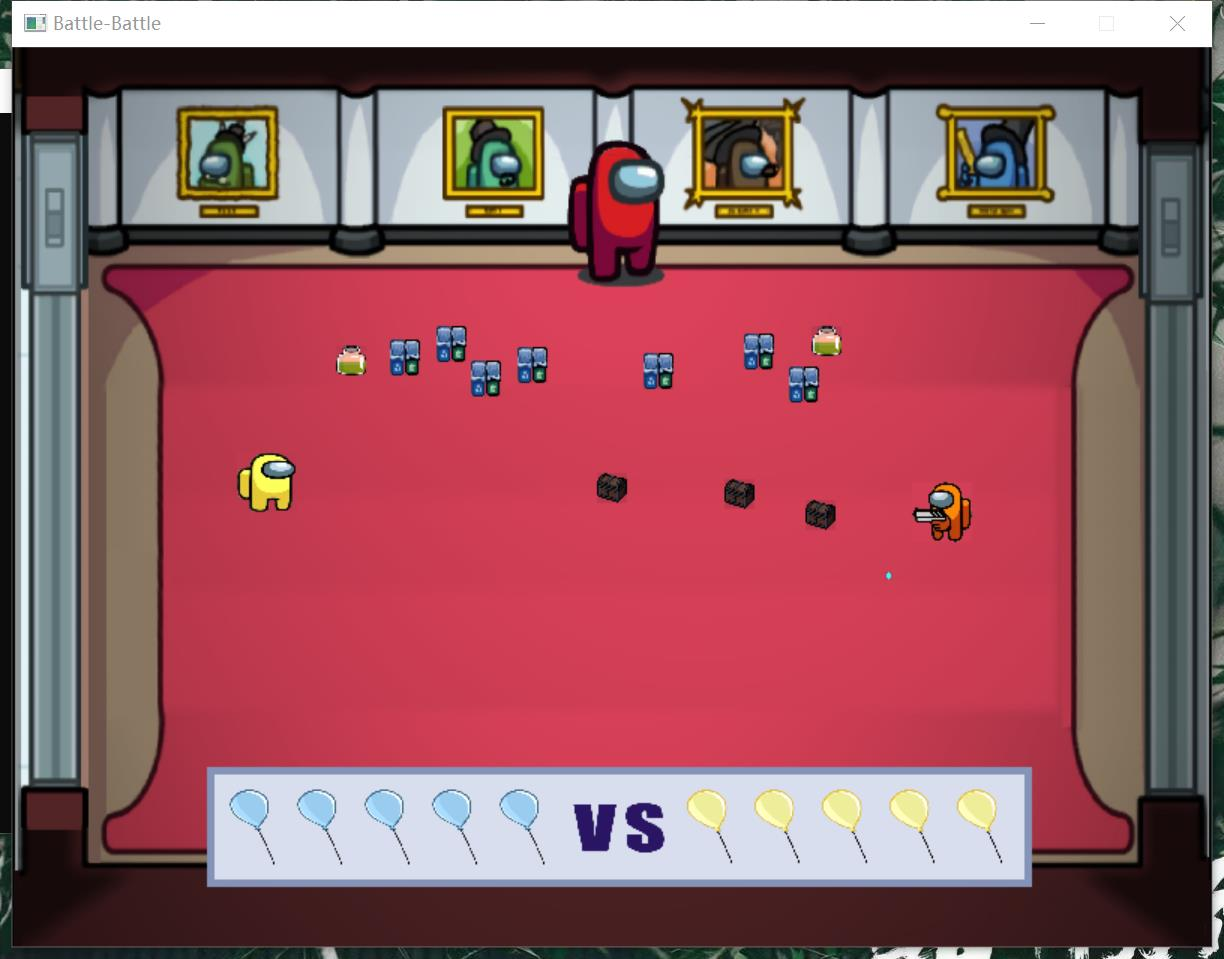
\includegraphics[width=0.8\textwidth]{images/4-12.jpg}
    \caption{Player1(黄色人物)发射子弹}% label 用来在文中索引
\end{figure}
\par
游戏规则:
\begin{itemize}
    \item 玩家每轮拥有一发子弹,在发出子弹且未装弹时,玩家只能通过“←”或“→”改变人物的移动方向;
    \item 当两名玩家均完成该轮射击后,双方同时填弹进入下一轮,填弹需要花费一定的时间。
    \item 在界面中央会随机出现若干道具,这些道具将给已发射的子弹提供属性加成,道具的功能为:\begin{itemize}
        \item 垃圾桶道具:当子弹射击到垃圾桶时,子弹会被垃圾桶弹射从而改变弹道方向;
        \item 药水道具:当子弹射击到药水道具时,子弹会得到增强,伤害提高至两点;
        \item 箱子道具:当子弹射击到箱子道具时,子弹的移动速度会降低,变化的子弹速度将影响另一位玩家的游戏节奏,从而提升对方躲避子弹的难度;
    \end{itemize}
\end{itemize}
\par
\begin{figure}[htbp]
    \vspace{13pt} % 调整图片与上文的垂直距离
    \centering
    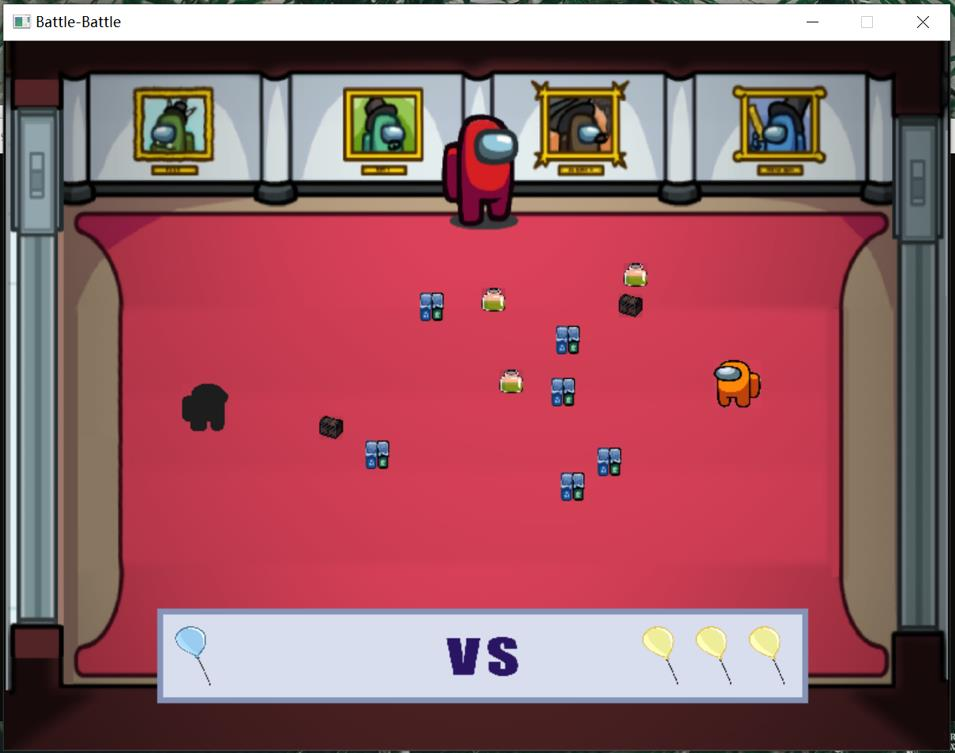
\includegraphics[width=0.8\textwidth]{images/4-13.jpg}
    \caption{Player1中弹的效果图}% label 用来在文中索引
\end{figure}
\par
当某一方的生命值小于等于0时,自动进入到游戏结算界面,游戏结束。
\par
\begin{figure}[htbp]
    \vspace{13pt} % 调整图片与上文的垂直距离
    \centering
    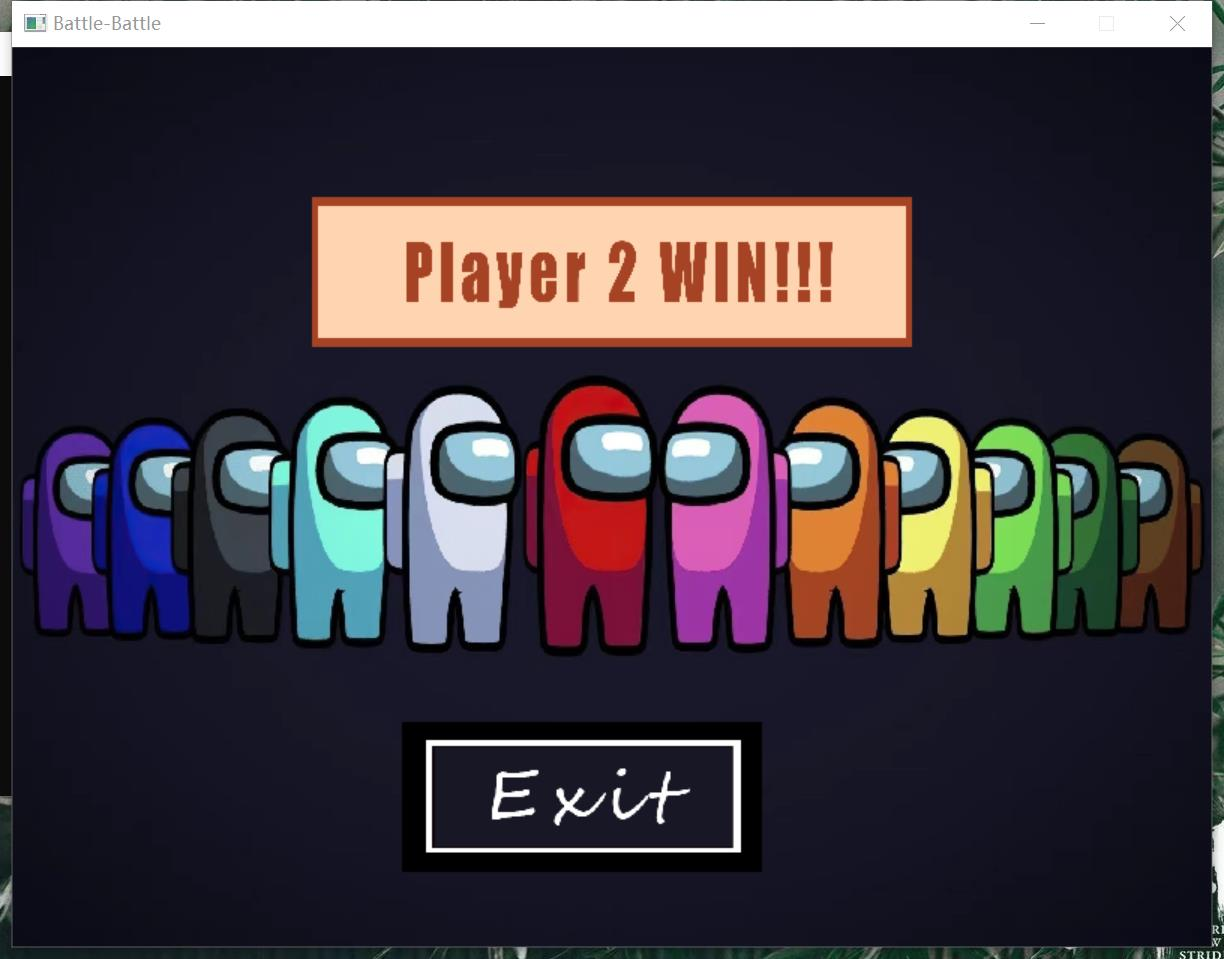
\includegraphics[width=0.8\textwidth]{images/4-14.jpg}
    \caption{Player2的获胜场景}% label 用来在文中索引
\end{figure}
\par
此时单击“Exit”即可关闭程序运行,退出游戏。


\chapter{总结心得}
\section{简要开发节点}
\begin{lstlisting}
    5.20:开会确定了游戏内容、结构以及功能,并且在Github创建项目仓库;完成了前端素材的制作和上传;
    5.30:完成了第一版结构的搭建以及前端界面的实现;
    5.31:实现游戏人物的动态移动、子弹的动态移动以及鼠标键盘响应事件的;
    6.1:完成了项目的重构;实现了中弹功能;
    6.2:完成了人物状态改变、生命值功能以及发弹填弹机制;
    6.5:实现了道具位置随机的效果;
    6.10:完成了三种道具的功能实现;
    6.11:完成击中机制的补充、结算界面的跳转以及一些bug的修复;完成项目文档的编写和代码的整理。
\end{lstlisting}
\section{小组人员分工}
王岩:完成了整体所用数据结构的完整定义,进行代码结构的二次重构以及确定,基本运行逻辑的确定,人物移动,子弹击中、碰撞的初始功能的完成,合作完成了道具随机初始化、击中判定等功能。
\par
杨汶锦:完成了人物状态改变、发弹填弹机制、生命值逻辑判定和生命条界面显示的代码实现;参与了人物中弹的实现;完成了项目的打包以及Latex报告格式规范。
\par
吴一凡:完成了代码整体框架的初次编写,实现了图片和音乐的载入,以及所有界面绘制逻辑,跳转逻辑,按钮逻辑等的编写,合作完成了子弹碰撞,道具随机初始化等功能。
\par
蒙思洁:完成了游戏音乐素材的寻找和图片素材的制作,参与了部分界面绘制逻辑、部分跳转逻辑的撰写,修正了游戏结束判定的逻辑,完成实验报告的框架设计和分解后的模块图绘制。
\section{小组成员心得}
\subsection{王岩}
用汇编来从头写游戏还是十分熬人的,虽然有前人的架构和好用的库,但是真的从头到尾确定数据结构、架构、逻辑过程等等,到一个个细节:理解一个个子函数的作用、一些复杂数据结构如汇编里结构体的调用等等还是非常掉头发的,以及对出其不意的debug还是依靠大家通力合作来解决。
\par
考试时间紧迫,没能对所有功能做完整实现,还是有点遗憾。但是整体实验收获了许许多多的编程经验,对于汇编语言的应用也更加熟练,收获也是很多的。
\subsection{杨汶锦}
由于时间原因,汇编上机作业的小组项目和个人项目几乎是并行的。在两者间不断学习汇编的语法知识、指令使用的细节。在本次小组作业中我们清晰地感受到了将实际需求一步步细分、转化逻辑实现并最终转化代码实现的过程,在项目的各个部分间寻求协调并在一次次调试中寻找逻辑不严谨的地方,整体的开发过程虽然还算顺利但还是令人影响深刻的。
\par
最终我们基本实现了构思初期对这个游戏的绝大部分功能,也对于汇编语言、汇编程序有了更加深刻的认识。在debug时对于一条条指令追本溯源地思考、对于自身逻辑地一遍遍验证,最终实现了这个游戏。感谢默契且给力的队友们!
\subsection{吴一凡}
通过此次汇编小组实验,我对于汇编语言程序设计有了更进一步的认知,学习到了如何使用汇编语言完成一个较大规模程序的编写。在实验初期,由于对于汇编语言结构的不熟悉以及对于代码整体框架的不了解,不知道应该如何组织好整个程序,但在查找了相关资料,并且不断尝试后,我们最终逐步搭起了整个程序的框架。同时由于对一些库函数的不了解,所以在代码编写初期,经常需要查找相关资料,学习如何正确的调用函数。
\par
同样,在整个代码编写过程中我们也遇到了许多问题,也在不断对游戏逻辑进行完善。例如图片无法正确显示,循环无法正确调用,子弹行进路径与预期不符,人物属性出现错误等等。但这些问题最终也都在不断改进,小组成员互帮互助下得以解决。完成了此次实验后,我也收获了许多经验,提高了自己汇编代码的编写能力。
\subsection{蒙思洁}
此次汇编小组的实验令我对汇编语言的了解更深一层,三个个人的小实验令我学到了汇编语言基础的语句操作,而本小组实验令我对汇编语言的开发过程有了更深的认知。通过对整体游戏的效果想象,我们能够首先绘制出游戏每个界面需要什么素材、控件,绘制出主题游戏部分每个素材它的作用是什么,设计它的实现方法;在游戏开发初期需要对素材进行寻找和处理,使其能够合适地被使用,在游戏开发中期需要划分逻辑结构,弄明白每个功能的实现需要哪几方面的共同作用;在游戏开发末期需要对游戏进行大量覆盖性的测试和修正,同时要对应初期设计好的目标来完善那些未完成的功能。
\par
在代码编写中,问题是不可避免的。不论是刚开始搭建框架代码时,基础的图片素材无法被调用、小组成员的环境配置版本不一带来的无法运行的bug;还是后期在测试过程中发现,道具没有正常发挥作用、子弹停留在空中不继续移动的问题、人物的生命值降为0以后不能正确弹出game\_over界面等问题。但是只要肯去钻研,在一行一行代码中捋逻辑,在一个一个重复出现的变量名称中判断它的变化情况,在通力合作之下,我们最终总是能解决这些问题。在这次实验中,队友们的积极沟通和高效合作是我们小组的游戏程序能够完成开发的最重要的组成部分!
\section{不足和展望}
整个项目借鉴了《微观战争》游戏的一部分游戏机制以及操作机制,我们在复现其机制的基础上设计了三种道具特效。
\par
由于整体的项目开发时间短,小组成员精力有限,游戏仍存在以下几方面的不足:
\begin{itemize}
    \item 整体项目采用单线程设计,在高并发操作的情况下可能出现卡顿、崩溃的情况;
    \item 游戏整体动效不够平滑,对于动画关键帧的选取不够准确,游戏看起来较为简单廉价;
    \item 游戏开发过程中的协同不够智能高效,未高效使用git等版本控制技术提高协同开发效率;
\end{itemize}
对于这个游戏,我们还有以下可实现的提高和展望:
\begin{itemize}
    \item 采用多线程重构游戏:由于本次游戏涉及到键盘输入、逻辑计算和动画实现,当出现大量计算或高频次并发键盘输入时,游戏可能会出现卡顿和崩溃的可能性;我们可以采用多线程的方式通过设置全局的标志变量来进行多个线程间的通信,从而提高游戏的鲁棒性;
    \item 补充游戏机制:还可以为游戏增加更加多元化的玩法和彩蛋。比如说,可以在正式游戏界面增加菜单功能,在菜单里可以调整游戏的进度和音乐等效果;可以在玩家中弹以后增加一些成就系统。
\end{itemize}
\section{写在最后}
本次小组项目的实现离不开小组成员的付出和钻研、离不开张全新老师课堂上细致认真的讲授、离不开在GitHub、Google贡献汇编开发技巧和问题解决方案的每一位前辈。感谢各位有形或无形的帮助,祝好!
% 结论:在结论相应的 TeX 文件处进行结论部分的撰写
%%%
% The BIThesis Template for Bachelor Graduation Thesis
%
% 北京理工大学毕业设计(论文)结论 —— 使用 XeLaTeX 编译
%
% Copyright 2020-2021 BITNP
%
% This work may be distributed and/or modified under the
% conditions of the LaTeX Project Public License, either version 1.3
% of this license or (at your option) any later version.
% The latest version of this license is in
%   http://www.latex-project.org/lppl.txt
% and version 1.3 or later is part of all distributions of LaTeX
% version 2005/12/01 or later.
%
% This work has the LPPL maintenance status `maintained'.
%
% The Current Maintainer of this work is Feng Kaiyu.
%
% Compile with: xelatex -> biber -> xelatex -> xelatex

\unnumchapter{结~~~~论}
\renewcommand{\thechapter}{结论}

\ctexset{
  section/number = \arabic{section}
}

% 结论部分尽量不使用 \subsection 二级标题,只使用 \section 一级标题

% 这里插入一个参考文献,仅作参考
本文结论……。\cite{李成智2004飞行之梦}

\textcolor{blue}{结论作为毕业设计(论文)正文的最后部分单独排写,但不加章号。结论是对整个论文主要结果的总结。在结论中应明确指出本研究的创新点,对其应用前景和社会、经济价值等加以预测和评价,并指出今后进一步在本研究方向进行研究工作的展望与设想。结论部分的撰写应简明扼要,突出创新性。阅后删除此段。}

\textcolor{blue}{结论正文样式与文章正文相同:宋体、小四;行距:22 磅;间距段前段后均为 0 行。阅后删除此段。}

% 参考文献:如无特殊需要,参考文献相应的 TeX 文件无需改动,添加参考文献请使用 BibTeX 的格式
%   添加至 misc/ref.bib 中,并在正文的相应位置使用 \cite{xxx} 的格式引用参考文献
% %%
% The BIThesis Template for Bachelor Graduation Thesis
%
% 北京理工大学毕业设计(论文)参考文献 —— 使用 XeLaTeX 编译
%
% Copyright 2020-2021 BITNP
%
% This work may be distributed and/or modified under the
% conditions of the LaTeX Project Public License, either version 1.3
% of this license or (at your option) any later version.
% The latest version of this license is in
%   http://www.latex-project.org/lppl.txt
% and version 1.3 or later is part of all distributions of LaTeX
% version 2005/12/01 or later.
%
% This work has the LPPL maintenance status `maintained'.
%
% The Current Maintainer of this work is Feng Kaiyu.
%
% Compile with: xelatex -> biber -> xelatex -> xelatex
%
% 如无特殊需要,本页面无需更改

% 参考文献开始
\unnumchapter{参考文献}
\renewcommand{\thechapter}{参考文献}

% 设置参考文献字号为 5 号
\renewcommand*{\bibfont}{\zihao{5}}
% 设置参考文献各个项目之间的垂直距离为 0
\setlength{\bibitemsep}{0ex}
\setlength{\bibnamesep}{0ex}
\setlength{\bibinitsep}{0ex}
% 设置单倍行距
\renewcommand{\baselinestretch}{1.2}
% 设置参考文献顺序标签 `[1]` 与文献内容 `作者. 文献标题...` 的间距
\setlength{\biblabelsep}{0.5mm}
% 设置参考文献后文缩进为 0(与 Word 模板保持一致)
\renewcommand{\itemcmd}{
  \addvspace{\bibitemsep} % 恢复 \bibitemsep 的作用
  \mkgbnumlabel{\printfield{labelnumber}}
  \hspace{\biblabelsep}}
% 删除默认的「参考文献 / Reference」标题,使用上面定义的 section 标题

% -------------------------------- 示例内容 ------------------------------------- %
\textcolor{blue}{参考文献书写规范}

\textcolor{blue}{参考国家标准《信息与文献参考文献著录规则》【GB/T 7714—2015】,参考文献书写规范如下:}

\textcolor{blue}{\textbf{1. 文献类型和标识代码}}

\textcolor{blue}{普通图书:M}\qquad\textcolor{blue}{会议录:C}\qquad\textcolor{blue}{汇编:G}\qquad\textcolor{blue}{报纸:N}

\textcolor{blue}{期刊:J}\qquad\textcolor{blue}{学位论文:D}\qquad\textcolor{blue}{报告:R}\qquad\textcolor{blue}{标准:S}

\textcolor{blue}{专利:P}\qquad\textcolor{blue}{数据库:DB}\qquad\textcolor{blue}{计算机程序:CP}\qquad\textcolor{blue}{电子公告:EB}

\textcolor{blue}{档案:A}\qquad\textcolor{blue}{舆图:CM}\qquad\textcolor{blue}{数据集:DS}\qquad\textcolor{blue}{其他:Z}

\textcolor{blue}{\textbf{2. 不同类别文献书写规范要求}}

\textcolor{blue}{\textbf{期刊}}

\noindent\textcolor{blue}{[序号]主要责任者. 文献题名[J]. 刊名, 出版年份, 卷号(期号): 起止页码. }

\printbibliography [type=article,heading=none] 

\textcolor{blue}{\textbf{普通图书}}

\noindent\textcolor{blue}{[序号]主要责任者. 文献题名[M]. 出版地: 出版者, 出版年. 起止页码. }
\cite{Raymer1992Aircraft}

\printbibliography [keyword={book},heading=none] 

\textcolor{blue}{\textbf{会议论文集}}

\noindent\textcolor{blue}{[序号]析出责任者. 析出题名[A]. 见(英文用In): 主编. 论文集名[C]. (供选择项: 会议名, 会址, 开会年)出版地: 出版者, 出版年. 起止页码. }
\cite{sunpinyi}

\printbibliography [type=inproceedings,heading=none] 

\textcolor{blue}{\textbf{专著中析出的文献}}

\noindent\textcolor{blue}{[序号]析出责任者. 析出题名[A]. 见(英文用In): 专著责任者. 书名[M]. 出版地: 出版者, 出版年.起止页码. }
\cite{luoyun}

\printbibliography [type=inbook,heading=none] 

\textcolor{blue}{\textbf{学位论文}}

\noindent\textcolor{blue}{[序号]主要责任者. 文献题名[D]. 保存地: 保存单位, 年份. }
\cite{zhanghesheng}
\cite{Sobieski}

\printbibliography [keyword={thesis},heading=none] 

\textcolor{blue}{\textbf{报告}}

\noindent\textcolor{blue}{[序号]主要责任者. 文献题名[R]. 报告地: 报告会主办单位, 年份. }
\cite{fengxiqiao}
\cite{Sobieszczanski}

\printbibliography [keyword={techreport},heading=none] 

\textcolor{blue}{\textbf{专利文献}}

\noindent\textcolor{blue}{[序号]专利所有者. 专利题名[P]. 专利国别: 专利号, 发布日期. }
\cite{jiangxizhou}

\printbibliography [type=patent,heading=none] 

\textcolor{blue}{\textbf{国际、国家标准}}

\noindent\textcolor{blue}{[序号]标准代号. 标准名称[S]. 出版地: 出版者, 出版年. }
\cite{GB/T16159—1996}

\printbibliography [keyword={standard},heading=none] 

\textcolor{blue}{\textbf{报纸文章}}

\noindent\textcolor{blue}{[序号]主要责任者. 文献题名[N]. 报纸名, 出版年, 月(日): 版次. }
\cite{xiexide}

\printbibliography [keyword={newspaper},heading=none] 

\textcolor{blue}{\textbf{电子文献}}

\noindent\textcolor{blue}{[序号]主要责任者. 电子文献题名[文献类型/载体类型]. 电子文献的出版或可获得地址(电子文献地址用文字表述), 发表或更新日期/引用日期(任选). }
\cite{yaoboyuan}

\printbibliography [keyword={online},heading=none] 

\textcolor{blue}{关于参考文献的未尽事项可参考国家标准《信息与文献参考文献著录规则》(GB/T 7714—2015)}

% 在使用时,请删除/注释上方示例内容,并启用下方语句以输出所有的参考文献
% \printbibliography[heading=none]

% 附录:在附录相应的 TeX 文件处进行附录部分的撰写
%%%
% The BIThesis Template for Bachelor Graduation Thesis
%
% 北京理工大学毕业设计(论文)附录 —— 使用 XeLaTeX 编译
%
% Copyright 2020-2021 BITNP
%
% This work may be distributed and/or modified under the
% conditions of the LaTeX Project Public License, either version 1.3
% of this license or (at your option) any later version.
% The latest version of this license is in
%   http://www.latex-project.org/lppl.txt
% and version 1.3 or later is part of all distributions of LaTeX
% version 2005/12/01 or later.
%
% This work has the LPPL maintenance status `maintained'.
%
% The Current Maintainer of this work is Feng Kaiyu.
%
% Compile with: xelatex -> biber -> xelatex -> xelatex

\unnumchapter{附~~~~录}
\renewcommand{\thechapter}{附录}

% 设置附录编号格式
\ctexset{
  section/number = 附录\Alph{section}
}

附录相关内容…

% 这里示范一下添加多个附录的方法:

\section{\LaTeX 环境的安装}
\LaTeX 环境的安装。

\section{BIThesis 使用说明}
BIThesis 使用说明。

\textcolor{blue}{附录是毕业设计(论文)主体的补充项目,为了体现整篇文章的完整性,写入正文又可能有损于论文的条理性、逻辑性和精炼性,这些材料可以写入附录段,但对于每一篇文章并不是必须的。附录依次用大写正体英文字母 A、B、C……编序号,如附录 A、附录 B。阅后删除此段。}

\textcolor{blue}{附录正文样式与文章正文相同:宋体、小四;行距:22 磅;间距段前段后均为 0 行。阅后删除此段。}

% 致谢:在致谢相应的 TeX 文件处进行致谢部分的撰写
% %%
% The BIThesis Template for Bachelor Graduation Thesis
%
% 北京理工大学毕业设计(论文)致谢 —— 使用 XeLaTeX 编译
%
% Copyright 2020-2021 BITNP
%
% This work may be distributed and/or modified under the
% conditions of the LaTeX Project Public License, either version 1.3
% of this license or (at your option) any later version.
% The latest version of this license is in
%   http://www.latex-project.org/lppl.txt
% and version 1.3 or later is part of all distributions of LaTeX
% version 2005/12/01 or later.
%
% This work has the LPPL maintenance status `maintained'.
%
% The Current Maintainer of this work is Feng Kaiyu.
%
% Compile with: xelatex -> biber -> xelatex -> xelatex

\unnumchapter{致~~~~谢}
\renewcommand{\thechapter}{致谢}

\ctexset{
  section/number = \arabic{section}
}

% 致谢部分尽量不使用 \subsection 二级标题,只使用 \section 一级标题

值此论文完成之际,首先向我的导师……

\textcolor{blue}{致谢正文样式与文章正文相同:宋体、小四;行距:22 磅;间距段前段后均为 0 行。阅后删除此段。}


\end{document}
